\documentclass[AMA,STIX1COL]{WileyNJD-v2}

\articletype{Article Type}%

\received{01 June 2018}
\revised{01 August 2018}
\accepted{01 August 2018}

\raggedbottom
\usepackage{subcaption}
\captionsetup[subfigure]{font=normalsize}

\usepackage{glossaries}
\makeglossaries

\begin{document}

\title{Open-source platforms for fast room acoustic simulations in complex structures}
%\title{This is the sample article title\protect\thanks{This is an example for title footnote.}}

\author[1]{Matthieu Aussal}

\author[2]{Robin Gueguen}



%\author[3]{Author Three}

\authormark{AUSSAL \& GUEGUEN}

\address[1]{\orgdiv{Centre de math\'ematique appliqu\'ees}, \orgname{\'Ecole Polytechnique}, \orgaddress{91128 Palaiseau, \country{France}}}

\address[2]{\orgdiv{Institut des Sciences du Calcul et des Donn\'ees}, \orgname{Sorbonne Universit\'e}, \orgaddress{Campus Pierre et Marie Curie - 4 place Jussieu, 75252 Paris Cedex 05 \country{France}}}




\corres{ \email{matthieu.aussal@polytechnique.edu}\\\email{gueguen.robin@gmail.com}}

%\presentaddress{This is sample for present address text this is sample for present address text}

\abstract[Summary]{
This article presents new numerical simulation tools, both for Matlab and Blender CAD software. Available in open-source under GPL 3.0 license, it uses a ray tracing / image-sources hybrid method to calculate room acoustics for large meshes. Performances are optimized to solve significant size numerical problems (typically more than 100,000 surface elements and about a million of rays). For this purpose, a \textit{Divide and Conquer} approach with a recursive octree structure has been implemented to reduce the quadratic complexity of the ray/element interactions to near-linear. Thus, execution times are less sensitive to mesh density, which allows complex geometry simulations. After ray propagation, a hybrid method leads to image-sources format, which can be visually analyzed to localize sound map. Finally, impulse responses are constructed from the image-sources and FIR filters are proposed natively over 8 octave bands, taking into account material absorption properties and propagation medium. This algorithm is validated by various comparison with theoretical test cases. Furthermore, an exemple on a complex case with the ancient theater of Orange is presented. 
}

\keywords{room acoustic, ray-tracing, image-sources, octree, Matlab, Blender, archeology, open-source}

\jnlcitation{\cname{%
\author{M. Aussal}, and
\author{R. Gueguen}, 
} (\cyear{2018}), 
\ctitle{Room acoustic measurement tool for complex geometry}, \cjournal{International Journal for Numerical Methods in Engineering}, \cvol{2018;00:1--6}.}

\maketitle

%\footnotetext{\textbf{Abbreviations:} ANA, anti-nuclear antibodies; APC, antigen-presenting cells; IRF, interferon regulatory factor}

% glossaire
%\section{Glossary\label{app1}}
%\newacronym{CAD}{CAD}{Computer-Aided Design}
%\newacronym{rir}{RIR}{\emph{Room Impulse response}}
%\newacronym{RT60}{$RT_{60}$}{\emph{Reveberation Time at $-60dB$}}
%\newacronym{orchestra}{\textit{orchestra}}{\emph{Semicircular (Roman) or circular (Greek) space between the stage and the first tier}}
%
%\gls{CAD}\\
%\gls{rir}\\
%\gls{RT60}\\
%\gls{orchestra} 

\section{Introduction}\label{sec1}
Today, digital technologies allow research to explore previously inaccessible areas, as virtual reality for archaeology. In this domain, many works focus on the visual restitution, but acoustic studies can reinforce researches to improve the understanding of the ancient world. For example, during the Roman Empire, architects have designed buildings also based on the sound propagation they wanted to achieve\cite{vitruve}. In this study, we focus on the ancient theater of Orange which has a significant size (100m wide), a complex geometry (decoration, gradins, colonnes, arcades ...) and which is open air. In a previous work, a complete mesh was designed using Blender CAD software (citer Blender), according to the most recent archeological knowledge \cite{theseRobin}. To be representative, this mesh has hundreds of thousands of elements (triangular faces), with complex shape (inserer figure maillage pour montrer la complexite). As this numerical model is now used by researchers to perform archeological hypothesis, we developed our own room acoustic software, directly integrated in the archeologists workflow. As the mesh size makes difficult the use of precise methods (FEM, BEM, ...), this software is based on a ray-tracing approximation, in order to compute fastly the full-band room impulse response (50 to 15000Hz). This tool has been developed following two steps. We first build a prototype using Gypsilab, an open source Matlab framework for fast prototyping (citer le papier gypsilab). This preliminary work was usefull to construct and validate ideas and algorithms. It conducts to the creation of a new toolbox, now added to the master branch of Gypsilab, and freely downloadable (citer adresse github). In a second step, all algorithms was retranscrypted in C++ using Qt Creator, leading to an autonomous library. A python interface was added, in order to use this library as a Blender plug'in. At the end, this plug'in allow archeologists to only work on Blender, modifying easily meshes and materials, run acoustic simulation and visualize results. \\
After reminders on acoustical energy propagation represented by ray-tracing, this paper gives implementation details for fast computation for large meshes. At the end, validation test cases are given and application on our modelization of the ancient theater of Orange is performed. 




\section{Acoustical energy modelization}\label{sec2}
\subsection{Continuous domain equation}

By modelling a point sound source as a localized pulse in space, the associated acoustical energy E(t) propagates \cite{jouhaneau} over time on a spherical surface $S(t)$, such that :
%
\begin{equation} 
E(t) = E_0 \int_{S(t)} \overrightarrow{I}(t).\overrightarrow{ds} \qquad \forall t > 0,
\end{equation}
%
with $E_0$ the initial energy and $\overrightarrow{I}(t)$ the acoustical intensity. According to the first principle of thermodynamics and by neglecting the effects of losses related to the absorption of the propagation medium, the acoustic energy is preserved over time. Thus, for a normalized punctual source :
%
\begin{equation} 
\int_{S(t)} \overrightarrow{I}(t).\overrightarrow{ds} = 1 \qquad \forall t > 0.
\end{equation}
%
After integration on the spherical surface $S(t)$, the infinitesimal acoustic intensity is written :
\begin{align} 
% \overrightarrow{I}(t) &= \frac{ \overrightarrow{d}(t)}{4\pi d(t)^3} \qquad \forall t > 0 \nonumber, \\
|| \overrightarrow{I}(t) || &= \frac{1}{4\pi d(t)^2} \qquad \forall t > 0,
\end{align}
%
reflecting that intensity decreases as the square of the distance to the source d(t). Integrating on a portion $\sigma(t)$ of the complete sphere $S(t)$, the energy is then carried by the solid angle $\Omega_{\sigma}$ :
%
\begin{equation}
E_{\sigma}(t) = E_0 \int_{\sigma(t)}  \frac{1}{4\pi  d(t)^2} ds = \frac{E_0}{4\pi}  \Omega_{\sigma}.
\label{eq_4}
\end{equation}
%
This last equation shows that the energy of a solid angle is constant over time and corresponds to a portion of the initial energy~$E_0$. Thus, subdividing $S(t)$ in $N$ portions $\sigma_i(t)$, the total energy can be decomposed as a sum of elementary energies, carried by solid angles $\Omega_i$, such as : 
%
\begin{equation}
E(t) = \sum_{i=1}^N E_i(t) = \frac{E_0}{4\pi}  \sum_{i=1}^N \Omega_i  \qquad \forall t > 0.
\label{eq_5}
\end{equation}
Ones can notice that $(\Omega_i)_{i\in[1,N] }$ is a directional basis, representing energy propagation by piecewise constant elements. Furthermore, for greater clarity, we definitively set in the following $E_0 = 1$.

\subsection{Discrete model}

To numerically represent the energy propagation, we have to discretize basis $(\Omega_i)_{i\in[1,N] }$ in (eq.~\ref{eq_5}). For this purpose, we define a \textit{ray} object composed by :
\begin{itemize}
\item An origin coordinate $x_i$,
\item A direction vector $\overrightarrow{u_i}$,
\item An energy value $E_i$.
\end{itemize}

For example, with an omnidirectional source, \textit{rays} are given by :
\begin{itemize}
\item The source coordinate ($x_i = x_s,~\forall i\in[1,N]$),
\item A unit sphere uniform sampling (e.g.~icosahedre subdivision, Fibonacci's rule \cite{fibonacci}, etc.),
\item An uniform energy repartition ($E_i = \frac{4\pi}{N},~\forall i\in[1,N]$).
\end{itemize}

To complete this approach, we have to define a discrete measure of energy propagation. To this end, we consider a $r$-radius measurement sphere $S(x_m, r)$, centered on $x_m$.  We can then add the contributions of the n rays that intersect this sphere to calculate the acoustic energy $E_m$ at point $x_m$ :

\begin{equation}
E_m \approx  \frac{1}{4\pi}  \sum_{i=1}^n E_i.
\end{equation}
In the particular case of an omnidirectionnal source, we have : 
\begin{equation}
E_m \approx  \frac{n}{N},
\end{equation}
which means that the measured energy $E_m$ is statistically represented by the ratio of the countered \textit{rays} to the total number of \textit{rays}.

\begin{figure}[t]
\centering
	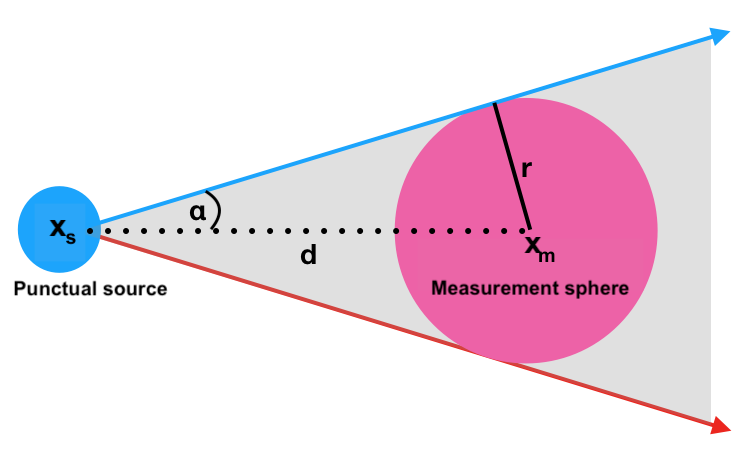
\includegraphics[width=0.6\linewidth]{schema_rayon}
	\caption{Representation of a $r$-radius measurement sphere centered in $x_m$, receiving energy from a sound source in $x_s$.}
	\label{schema_rayon}
\end{figure}

Moreover, applying the continuous model (eq.~\ref{eq_4}), the measured energy is given by :
\begin{equation}
E_m = \frac{1}{4\pi}  \Omega_m,
\end{equation}
where $\Omega_m$ is a solid angle of a cone of revolution (see fig. \ref{schema_rayon}), such as :
\begin{equation}
\Omega_m = 2\pi(1-\cos{\alpha}).
\end{equation}
Following the figure \ref{schema_rayon} :
\begin{equation}
\Omega_m = 2\pi \left( 1 - \sqrt{1-\frac{r^2}{d^2}} \right)
\end{equation}
and considering $\frac{r}{d} \ll 1$, 
\begin{equation}
\Omega_m = \pi \frac{r^2}{d^2}.
\end{equation}
At the end, 
\begin{equation}
E_m \approx  \frac{n}{N} \approx  \frac{\pi r^2}{4\pi d^2}.
\label{eq_12}
\end{equation}
To ensure the existence of this last approximation, at least one \textit{ray} have to be measured ($n\geq1$). Thus, fixing a measurement radius r, approximation (\ref{eq_12}) gives a maximum validity range of the discrete model :  
\begin{equation}
	d \leq \frac{r}{2}\sqrt{\frac{N}{n}}.
\end{equation}
In addition, figure \ref{energie} shows how this modelization fills with distance between source and measures. The accuracy of the measurement depends strongly on the number of  \textit{rays} counted, then, the more $n$ increases, the more accurate will be the measurement. Nevertheless, in practice, values for a short distance between the source and the measurement sphere represent direct sound and first reflections, whereas long distances describe the diffuse field. Under this assumption, we can consider this model acceptable for all $n\geq1$. 

\begin{figure}[t]
\centering
	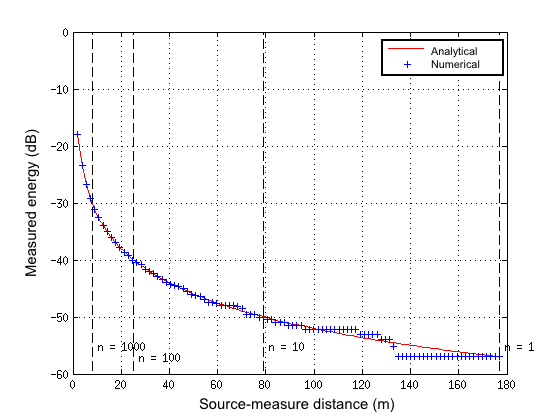
\includegraphics[width=0.8\linewidth]{energie.png}
	\caption{Measured energy (dB) in function of distance between $x_s$ and $x_m$ in meter for $r = 0.36$m and $N = 10^6$. Blue crosses stand for the statistical measure $f(r) = \frac{n(r)}{N}$ and red ligne the analytic function $f(r) = \frac{\pi r^2}{4\pi d^2}$.}
	\label{energie}
\end{figure}

%
\begin{figure}[b]
	\centering
	\begin{subfigure}{0.5\textwidth}
		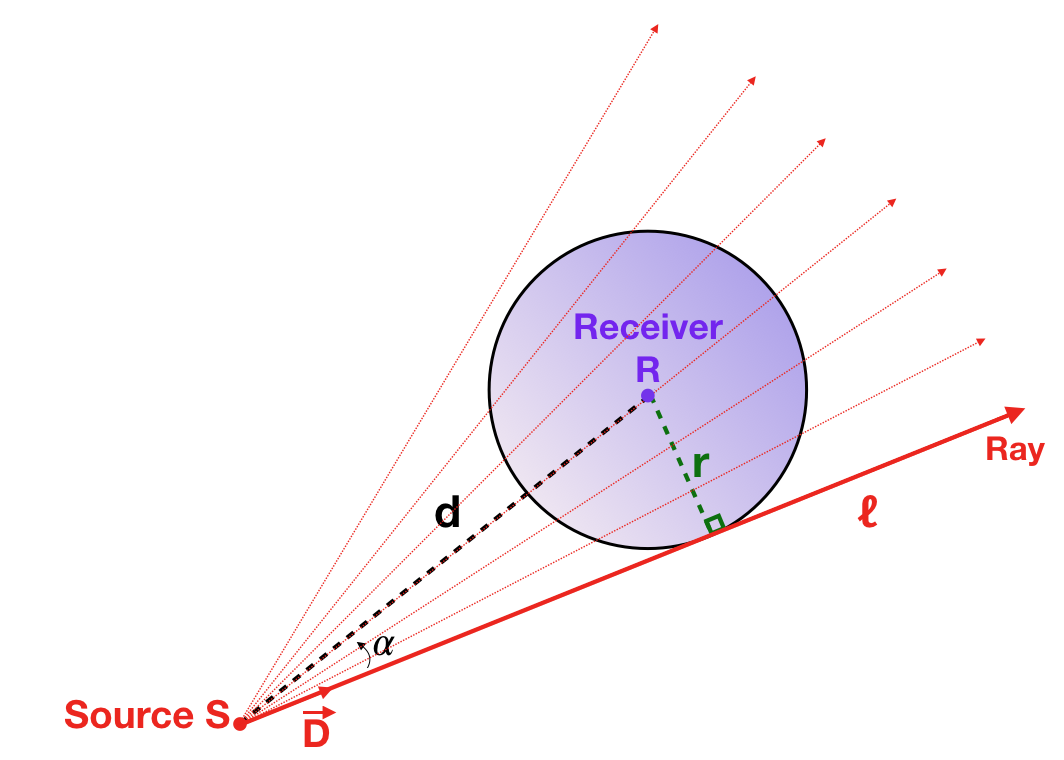
\includegraphics[width=\textwidth]{rays}
		\caption{Representation of \textit{rays} mesure by a receiver. }
		\label{rays}
	\end{subfigure}	
	\qquad
		\begin{subfigure}{0.4\textwidth}
%		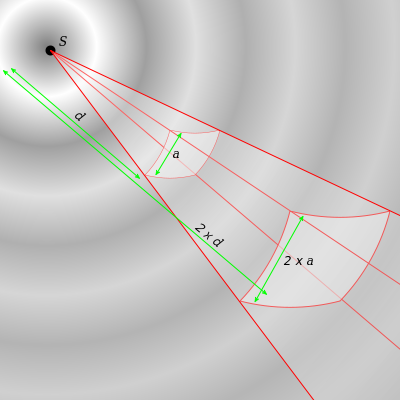
\includegraphics[width=\textwidth]{flux}
%		\caption{Representation of the distribution of the energy flow in the propagation of a spherical wave.}
%		\label{flux}
	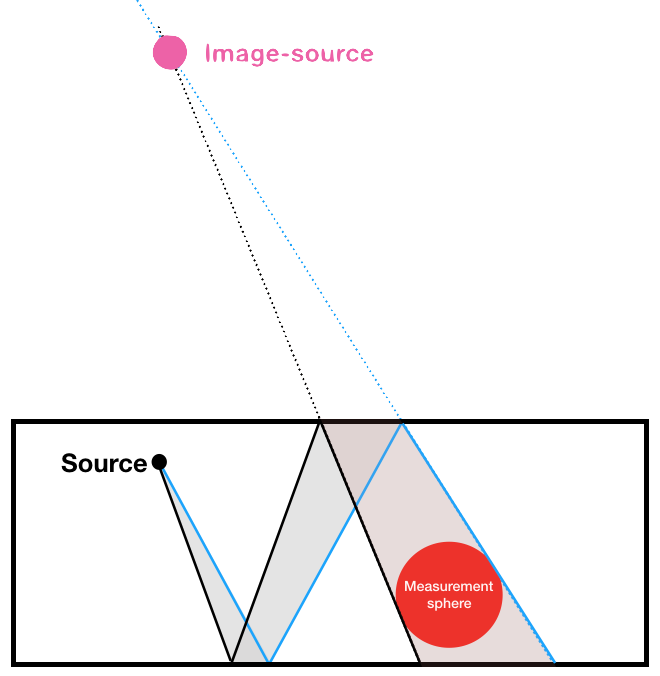
\includegraphics[width=\linewidth]{schema_SI}
	\caption{Sketch of the creation of an image-source by successive reflections of a ray on the walls of a room}
	\label{schema_SI}
	\end{subfigure}
	\caption{Acoustic emission from a point source.}
\end{figure}
%Example for bibliography citations cite\cite{Taylor1937}, cites\cite{Knupp1999,Kamm2000}



\subsection{Presence of an obstacle}
For the case of acoustic propagation in presence of an obstacle, we choose to only consider specular reflections (Snell-Descartes laws). Indeed, this approximation is suitable when surfaces are large in comparaison to wavelengths, because diffraction effects can be neglected \cite{jouhaneau}. For a room, this condition is reached if :
\begin{equation}
ka \gg 1, 
\end{equation}
with $k$ the wave number and $a$ the characteristical diameter of the room \cite{hautes_freq}. This approach is currently used by room acoustic softwares (e.g. \textit{Odeon} \cite{odeon}, \textit{Grasshopper} \cite{grasshopper}, etc.) regarding to audible frequency range (62,5 to 15000Hz). In particular, as the Theater of Orange has a characteristical diameter about 50 meters, the high frequency approximation is reached. 

Following the discrete model, when an incident \textit{ray} collides a flat surface, a reflected \textit{ray} is generated from the collision point. Noting $\overrightarrow{u_i}$ the direction vector of the incident  \textit{ray}, the reflected direction vector $\overrightarrow{u_r}$ is defined by :
\begin{equation}
\overrightarrow{u_r} = (\overrightarrow{u_i} \cdot \overrightarrow{T})\overrightarrow{T} - (\overrightarrow{u_i} \cdot \overrightarrow{n})\overrightarrow{n},
\end{equation}
with $\overrightarrow{T}$ the tangent basis and $\overrightarrow{n}$ the normal vector of the surface. Moreover, the energy of the reflected \textit{ray} is obtained by :
\begin{equation}
E_r(f) = E_i(f)(1 - \alpha(f)),
\end{equation}
with $\alpha(f)$  the absorption coefficient of the surface, function of the frequency $f$. Practically, the absorption coefficients are often given per octave bands and can be found in various databases. In Gypsilab and ..., both use the open access \textit{Odeon} database \cite{odeon} defined on eight octave bands (see table \ref{tab_coeff_abs}). 

Finally, considering wall absorption, energy measured statistically (eq. \ref{eq_12}) is extended by :
\begin{equation}
E_m(f) \approx  \frac{n}{N}(1 - \alpha(f)),
\end{equation}
generalizable to :
\begin{equation}
E_m(f) \approx  \frac{n}{N}\prod_{j=1}^{m}(1 - \alpha_j(f)),
\label{eq_18}
\end{equation}
in the case of $m$ reflexions.

\begin{table}
%\footnotesize
\centering
	\begin{tabular}{| c | m{2.5cm} | *{8}{c|}}
		\hline
		Reference & Material name & 62,5Hz & 125Hz & 250Hz & 500Hz & 1kHz & 2kHz & 4kHz & 8kHz \\
		  \hline
		  \hline
		   1 & 100\% absorbent & 1 & 1 & 1 & 1 & 1 & 1 & 1 & 1 \\
		   \hline
		2 & 100\% reflecting & 0 & 0 & 0 & 0 & 0 & 0 & 0 & 0 \\
		   \hline
		107 & Concrete block, coarse\footnotemark & 0.36 & 0.36 & 0.44 & 0.31 & 0.29 & 0.39 & 0.25 & 0.25 \\
		   \hline
		3000 & Hollow wooden podium\footnotemark & 0.4 & 0.4 & 0.3 & 0.2 & 0.17 & 0.15 & 0.1 & 0.1 \\
	     \hline
	 \end{tabular}
	\caption{Examples of absorption coefficient given in the onligne \textit{Odeon} database \cite{odeon}.}
	 \label{tab_coeff_abs}
\end{table}
\addtocounter{footnote}{-1}
\footnotetext{Harris, 1991}
\addtocounter{footnote}{1}
\footnotetext{Dalenback, CATT}


\subsection{Image-sources}
Although the extended formulation (eq. \ref{eq_18}) may be sufficient to generate room acoustic data, we also construct images-sources from the path of \textit{rays}. To this end, when \textit{rays} intersect a measurement sphere and following the reverse return principle, they are retro-propagated along the last direction vector. Thus, from this measurement sphere, \textit{rays} focus on punctual images-sources (see fig. \ref{schema_SI}). Each image-source is then located relatively to the listener and carry an energy according to equation (\ref{eq_18}). By noting $(x_s)_{s \in [1, N_s]}$ the relative position of the $N_s$ image sources and $(E_s)_{s \in [1, N_s]}$ the associated energy, couples $(x_s;E_s(f))_{s \in [1, N_s]}$ contain many useful informations for room acoustic analysis and auralization. 

First of all, relative distance of each source image $(d_s)_{s \in [1, N_s]}$ can be computed. This distances should be used to compute air absorption, adding a term in the equation (\ref{eq_18}) :
\begin{equation}
E_s(f) \approx  \frac{n}{N}  e^{-\beta(f) d_s}  \prod_{j=1}^{m}(1 - \alpha_j(f)),
\label{eq_19}
\end{equation}    
with $\beta(f)$ a frequency dependent coefficient (ref norme). Furthermore, fixing the sound celerity $c$, room impulse response can be generated, converting each distances $d_s$ in time of arrival. Taking care to convert energy into sound pressure ($p = \sqrt{E}$), finite impulse response can be generated and analyzed using standard metrics (e.g. $T_{30}$, $C_{80}$, $D_{50}$, etc.). For auralization, this room impulse response is convolved with an audio signal in order to listen the acoustical rendering. In particular, this convolution can involve relative position of predominant images sources, in order to realize a spatialized auralization with multichannel or binaural renderers. Finally, to complete acoustic studies with visual analysis, images sources can be projected on the room used for computation to see where are located listened reflections (see last impact on fig. \ref{schema_SI}).



\section{Implementation}
\subsection{Standard algorithm}
As standard principles are introduced, we focus now on the numerical implementation of an acoustic render by ray-tracing. Before any room acoustic computation, a numerical room has to be modelized with surfaces and materials.  that the model is meshed by flat triangularization.

 using simplex triangulation,   


~\\~\\
beam not measurable anymore

\subsection{Tree-base acceleration}

\section{Numerical validation}
\subsection{Shoes box (modele complet)}
\subsection{Energy conservation (sphere reflechissante)}

\section{Application to Orange theater}

\section{Conclusion}





\section{Hybride Ray-Tracing / Image-Source methode}\label{sec3}
\subsection{Ray-tracing \cite{raytracing}}

The method developed aims to propagate rays from a point source. A ray is define with the following equation (see fig .\ref{rays}) :
\begin{equation}
\overrightarrow{R}(d) = O + \overrightarrow{D}.d,
\end{equation}
where :
\begin{itemize}
\item $O$ is the origine of the ray,
\item $\overrightarrow{D}$ is the unitary orientation vecteur.
\end{itemize}


Once convert into cartesian coordinates and normalized we can test the intersection with the triangles of the mesh. The mesh elements have to be triangle with normales directed towards the inside of the room. By using the Moller-Trumbore fast algorithm \cite{moller}, for  each ray we can find the points T intersecting triangles, such as :

\begin{equation} \label{eq_2moller}
T(u,v) = (1-u-v)V_0 + uV_1 + vV_2 = O + D.d,% \ \ \ \footnotemark
\end{equation}
%\citefnt[eq. 2]{moller}
%
with $(u,v)$ the barycentric coordinates such as :
\begin{equation}
   \left \{
   \begin{array}{r c l}
u & \geqslant & -\epsilon,  \\
v & \geqslant & -\epsilon,  \\
(u+v) & \leqslant & 1+\epsilon,
   \end{array}
   \right .
\end{equation}
where $\epsilon = 10^{-5}$ to avoid rounding errors due to machine precision (float). This can be written : 
\begin{equation}
	\begin{bmatrix}
 	 d \\
	 u \\
	 v
	\end{bmatrix}
	=
	\frac{1}{
 	  (D \times E_2).E_1
	}
	\begin{bmatrix}
 		  (T \times E_1).E_2
 \\ 
 		  (D \times E_2).T
 \\
 		  (T \times E_1).D
	\end{bmatrix}	.
\end{equation}
with : 
\begin{equation}
   \left \{
   \begin{array}{r c l}
E_1 &=&  V_1-V_0,  \\
E_2 &=&  V_2-V_0,  \\
T &=& O - V_0.
   \end{array}
   \right .
\end{equation}
%
The good intersection is the one whose the distance $d$ between the origin of the ray and the intersection point T is the shortest. The rays can then be reflected on the face as on a mirror to find the new orientation vector :%(see fig. \ref{rayRefl}) :
\begin{equation}
\overrightarrow{r} - \overrightarrow{i} = 2 \times (-\overrightarrow{i}.\overrightarrow{n})\overrightarrow{n}.
\end{equation}
with : 
\begin{itemize}
\item $\overrightarrow{r}$ : the reflected ray,
\item $\overrightarrow{i}$ : the incident ray,
\item $\overrightarrow{n}$ : the normal of the face.
\end{itemize}

%\begin{figure}
%\centering
%	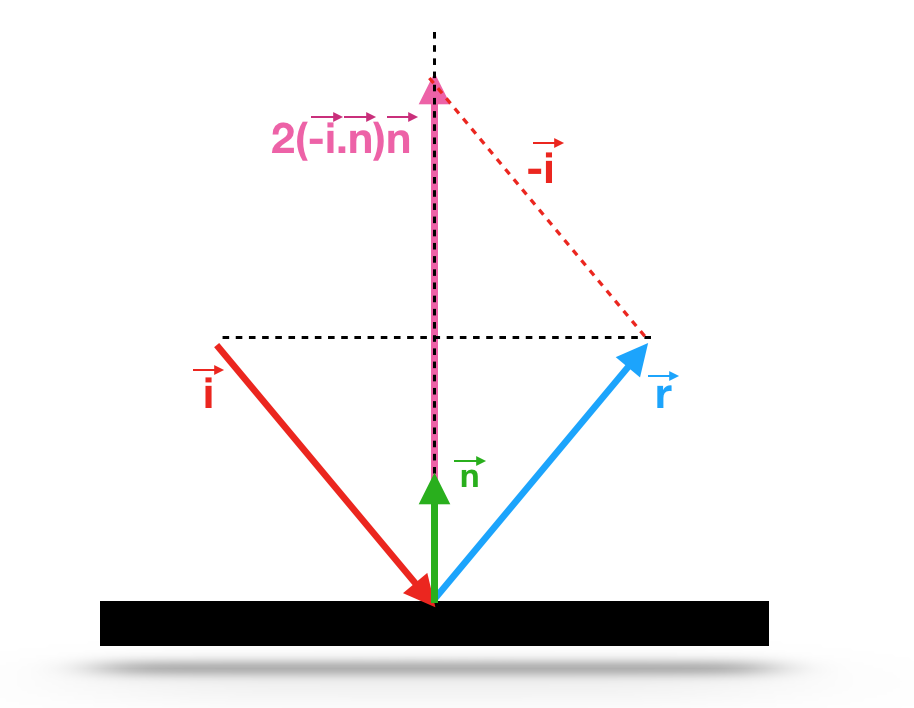
\includegraphics[width=0.4\linewidth]{rayRefl}
%	\caption{Calculation of a reflected ray from an incident ray and a normal ray}
%	\label{rayRefl}
%\end{figure}

Once we know the elements met be each ray we can update their energies. Each triangle carries an an absorption coefficient $\alpha_i$ for every octave band from 62,5Hz to 8kHz (so 8 bands) (see exemple on table \ref{exempleOdeon}). Moreover, we take into account the atmospheric attenuation. The energy of a ray is :
\begin{equation}
E_{i} =  \frac{1}{N} \times \prod_{j=0}^{k}{(1-\alpha_{i,j})} \times e^{-m_i . d_{tot}},
\end{equation}
with : 
\begin{itemize}
\item $E_{i}$ : the energy carried by the ray on the i-th frequency band,
\item $E_{0}$ : the total energy,
\item $k$ : the total number of faces encountered by the rays during its propagation,
\item $j$ : the index of the face encountered par the ray,
\item $m_i$ : the air absorption coefficient in the i-th frequency band (according to the norm ISO-9613),
\item $ d_{tot}$ : the total length of the ray from the source to the center of the receiver.
\end{itemize}


\subsection{Image-sources}

At each ray bounce, we check if the rays intersect the receiver-sphere. First we check if the origine point $O$ of the ray is include in the R-center and r-radius receiver :
\begin{equation}
||\overrightarrow{OR}|| \leqslant r,
\end{equation}
%
If not, we check the direction of the ray :
\begin{equation}
\cos{\alpha} \geqslant 0,
\end{equation}
with $\alpha$ the angle between the ray $\overrightarrow{D}$ and $\overrightarrow{OR}$. Then we check if the ray is long enough to reach the receiver :

\begin{equation}
||\overrightarrow{OR}|| \leqslant d,
\end{equation}
%
To finish, we check if the ray intersect the receiver-sphere :

\begin{align}
\sin{\alpha} \times ||\overrightarrow{OR}||  \leqslant r 
\quad \Rightarrow \quad
\alpha  \leqslant \arcsin{\frac{r}{||\overrightarrow{OR}||}}
\end{align}

If the ray does indeed intersect the receiver, an image-source is generated (see fig. \ref{schema_SI}). This is the image of the sound source relative to all the walls encountered by the ray. The image-source $I_S$ is located in space by back-propagation of the ray from its last origin point O :

\begin{equation}
\overrightarrow{I_S O} = \overrightarrow{D}.d_{tot} \qquad \Rightarrow \qquad I_S = O - \overrightarrow{D}.d_{tot},
\end{equation}
where 
\begin{itemize}
\item $\overrightarrow{D}$ is the last unitary orientation vector of the ray,
\item $d_{tot}$ is the total distance travelled by the ray from the original source S to the point O.
\end{itemize}

%\begin{figure}
%\centering
%	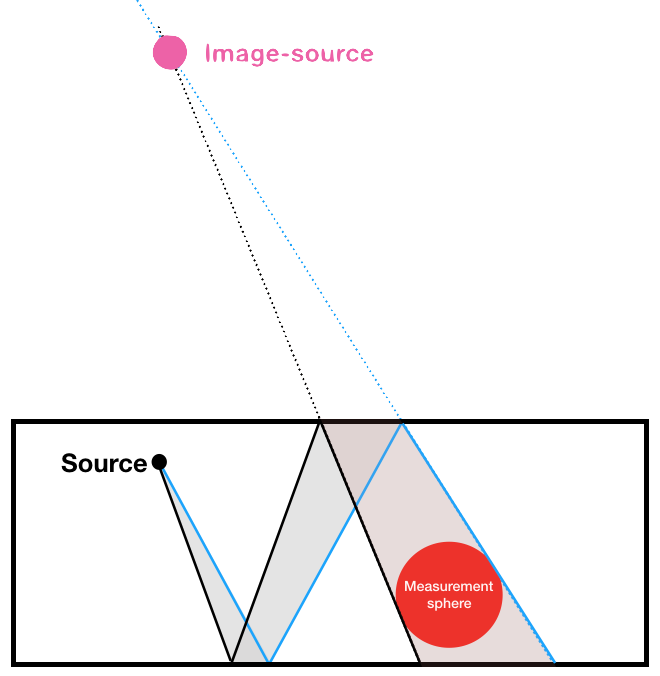
\includegraphics[width=0.3\linewidth]{schema_SI}
%	\caption{Sketch of the creation of an image-source by successive reflections of a ray on the walls of a room}
%	\label{schema_SI}
%\end{figure}

The positions of the image-sources allow to know the time it takes for the signal to arrive to the receiver :

\begin{equation}
t_{I_S} = \frac{||\overrightarrow{I_S O}|| + ||\overrightarrow{OR}||}{v}.
\end{equation}
with $v$ the sound speed in the medium (air : $v=340m/s$). The room impulse response can be generated for each octave band at a certain sampling frequency $f_s$ such as :

\begin{align}
E_{i} =  \sum{E_j},
\end{align}
with : 
\begin{itemize}
\item  the integer part of the product $(t_j \times f_s) = i$,
\item$E_{i}$ : the energy of the $i^{th}$ sample,
\item$E_j$ and $t_j$ : respectively the energy and travel time of the $j^{th}$ image-source.
\end{itemize}



%\newpage

\section{Algorithm's optimisation}\label{sec4}
\subsection{Presentation}

The algorithm has iteration loops with different complexities. There are three main steps which depend on the number of mesh elements $M$ and the number of rays emitted $N$ :\begin{itemize}
\item the mesh loading,
\item the intersection between rays and faces,
\item the image-sources creation.
\end{itemize}

The mesh loading depends only on the number of elements and is done only once at the beginning of the algorithm. The image-sources creation depends only on the number of rays and is done until the stop threshold is reached. The most critical stage is the intersection rays/faces because each ray has to be tested with each face and the loop is repeated until the stop threshold is reached. The complexity of this operation is quadratic in $O(N\times M)$. For a significant number of mesh elements ($>100~000$ for the Orange theater) and a lot of rays (necessary to make the measurement accurate) the calculation time is very long, which makes the tests tedious. To alleviate this problem we have developed a fast algorithm based on a "Divide and Conquer" approach based on Octree spatial cutting \cite{greengard}.

\begin{figure}[h]
\centering
\begin{subfigure}{0.52\textwidth}
	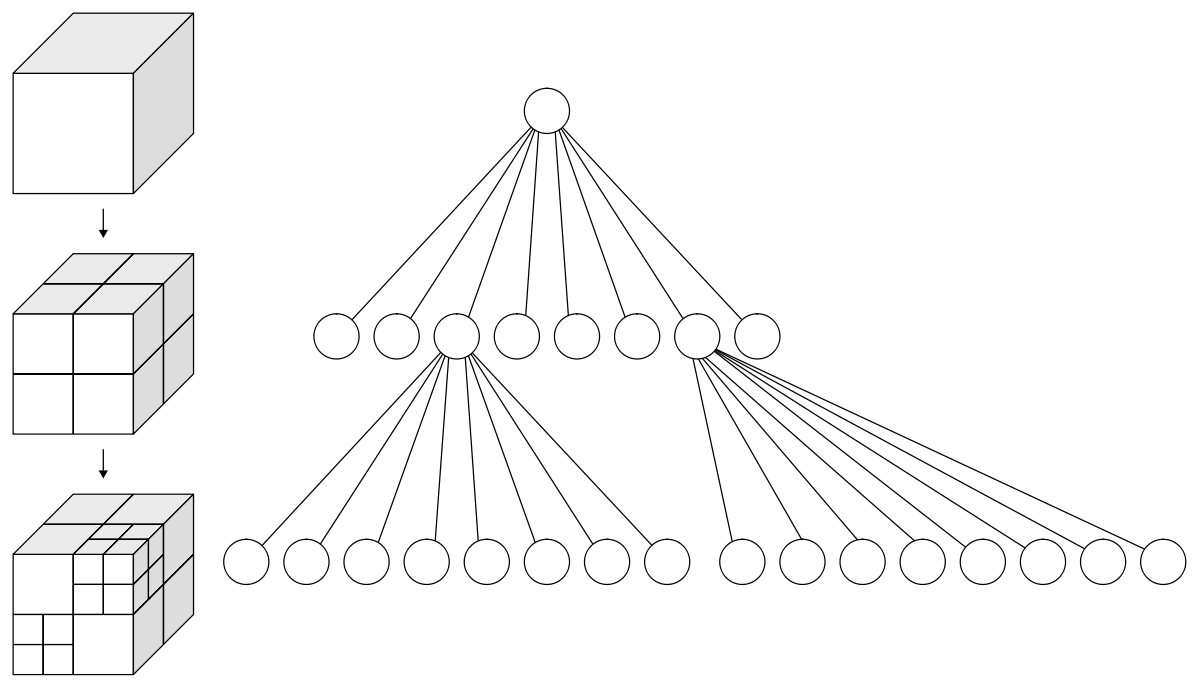
\includegraphics[width=\linewidth]{octree}
	\caption{Illustration of the Octree principle.}
	\label{octree}
	\end{subfigure}
	\begin{subfigure}{0.35\textwidth}
		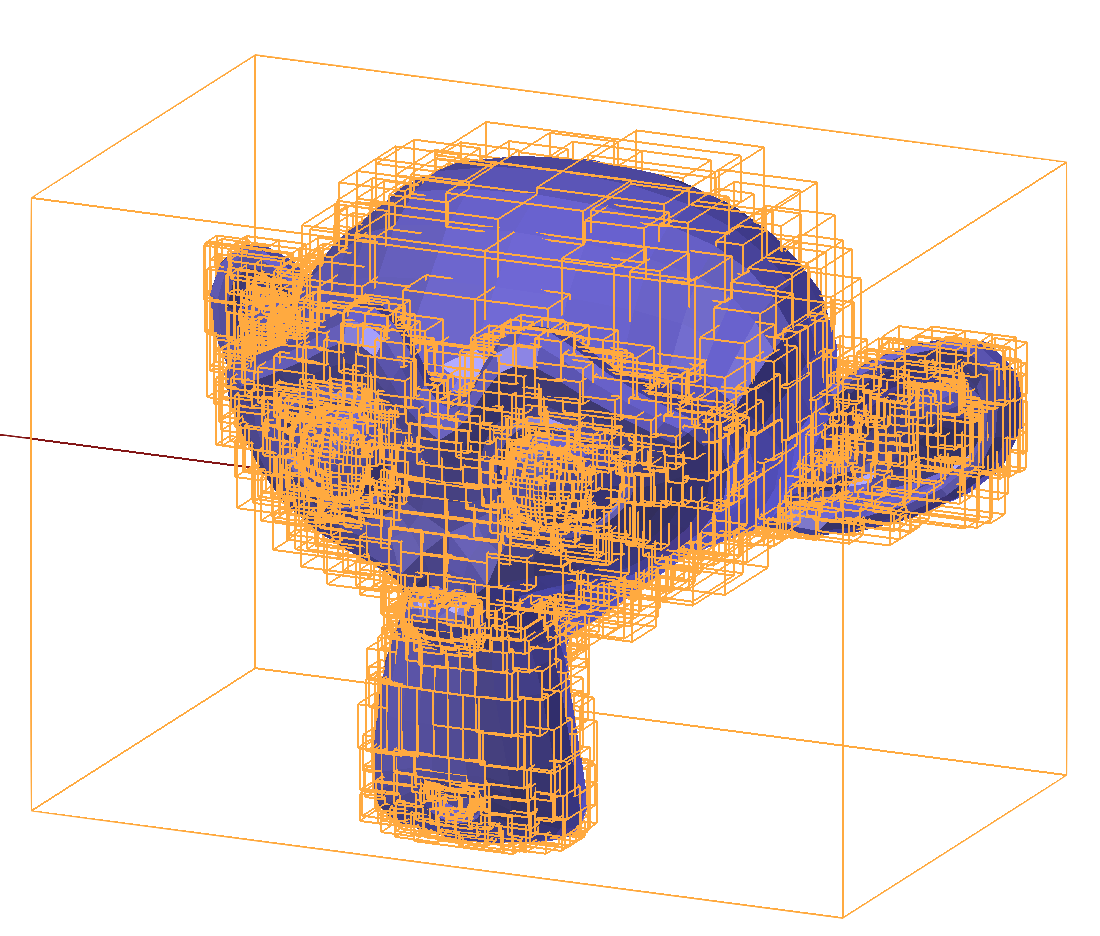
\includegraphics[width=\linewidth]{octreeSuzanne}
		\caption{Octree around an arbitrary mesh}
		\label{octreeSuzanne}
	\end{subfigure}
	\caption{Illustration of an Octree.}
	%\label{octree}
\end{figure}

The general principle consists in creating a cubic box called a "mother-box" containing all the mesh elements, i.e. all the triangular faces. This mother-box is then subdivided to create eight "daughter-boxes" of identical size which themselves will be subdivided into eight daughter-boxes, etc. (see fig. \ref{octree}). Recursively, each mother-box element will be stored in the daughter-box that contains it. In this way, you descend into the tree structure until a stop condition is reached. Typically, the octree stops when no more daughter-boxes contain more than $n$ items. The boxes are therefore refined in the same way as the mesh (see fig. \ref{octreeSuzanne}) since empty boxes do not generate daughter-boxes.

If we name \textit{item} a ray or a triangular face of the mesh and \textit{operation} the storage in a box, we can calculate the number of \textit{operations} to have only one \textit{item} per box. We place ourselves in the case where the \textit{items} are distributed in a uniform way in space. At level-0 all the $N$ \textit{items} are in the root-box. At level-1 we test each daughter-box with each \textit{item} and we have $8N$ \textit{operations}. At the next level each daughter-box become a mother-box and we can apply the same calculation to obtain :
\begin{center}
$8\times 8\times \frac{N}{8}$ = $8N$ \textit{operations}.
\end{center}
because each mother-box only count $\frac{N}{8}$ \textit{items}. Then, at level-p we will need  :
%
\begin{equation} \label{operation}
8^p\frac{N}{8^{p-1}} = 8N \ \textit{operations}.
\end{equation}
%
and the total number of \textit{operations} is $p\times 8N$.

Moreover we said that their is only one \textit{item} per box, so there are as many boxes as there are \textit{items}. We can write :
%
\begin{align}  \label{nbEtage}
8^p &= N \nonumber, \\
p.\ln{8} &= \ln{N} \nonumber, \\
p &= \frac{1}{\ln{8}}\ln{N}.
\end{align}
%
The total number of operation is then :
\begin{equation}
C = p.8N = \frac{8N}{\ln8}\ln{N}.
\end{equation}
%
Within the algorithm, instead of testing all rays with all faces, we test N times one ray with one face. The number of linear operations is :
\begin{equation}
C_{tot} =  \frac{8N}{\ln8}\ln{N} + N.
\end{equation}
which is faster than $N^2$ for $N>>1$.

In practice we will be able to stop the octree before arriving at only one element per box. Typically, if we stop the octree at $n$ elements per box the total number of operation become :
\begin{align}
C_{tot} &= \frac{8N}{\ln8}\ln{N} - \frac{\ln n }{\ln8}8N + n^2, \\
 &= aN\ln{N} +bN + c. \nonumber
\end{align}
with (a, b, c) some constants. So $n$ needs to be very small in front of $N$ to preserve the performance.

Note that when the distribution of items is not uniform the demonstration is more complicated but the calculation times remain substantially similar.

\subsection{Implementation}


To store the triangular faces in the box we test if the center of the face belongs to the box. Once each center has been store in the leaves of the octree (i.e the last boxes of the branches) we resize the leaves to embody the whole faces they contains. To test if a ray cross a box we use a pass/fail algorithm conceived for Axis-Aligned-Bounding-Box \cite{AABB}. This kind of box allow to simplify a lot the computation. 
%can be defined by six plans $\left[ X_{min}, X_{max}, Y_{min}, Y_{max}, Z_{min}, Z_{max} \right] $. If the ray equation is :
%\begin{equation}
%f(t) = D \times t + O
%\end{equation}
%with :
%\begin{itemize}
%\item $D$ : the orientation vector of the whose coordinates are $(D_x ; D_y ; D_z)$,
%\item $O$ : the origin point of the ray whose coordinates are $(O_x ; O_y ; O_z)$,
%\end{itemize}
%we can express the intersection point by this following system :
%\begin{align*}
%X_{min} &= x_0 \times D_x + O_x 	& \Rightarrow 	& &	 x_0 = \frac{X_{min} - O_x}{D_x}, \\
%X_{max} &= x_1 \times D_x + O_x 	& \Rightarrow 	& &	x_1 = \frac{X_{max} - O_x}{D_x}, \\
%Y_{min} &= y_0 \times D_y + O_y 	& \Rightarrow	& &	y_0 = \frac{Y_{min} - O_y}{D_y}, \\
%Y_{max} &= y_1 \times D_y + O_y 	& \Rightarrow	& &	y_1 = \frac{Y_{max} - O_y}{D_y}, \\
%Z_{min} &= z_0 \times D_z + O_z	& \Rightarrow 	& &	z_0 = \frac{Z_{min} - O_z}{D_z}, \\
%Z_{max} &= z_1 \times D_z + O_z 	& \Rightarrow 	& &	z_1 = \frac{Z_{max} - O_z}{D_z}. 
%\end{align*}
%%
%\begin{figure}
%\centering
%	\begin{subfigure}{0.4\textwidth}
%		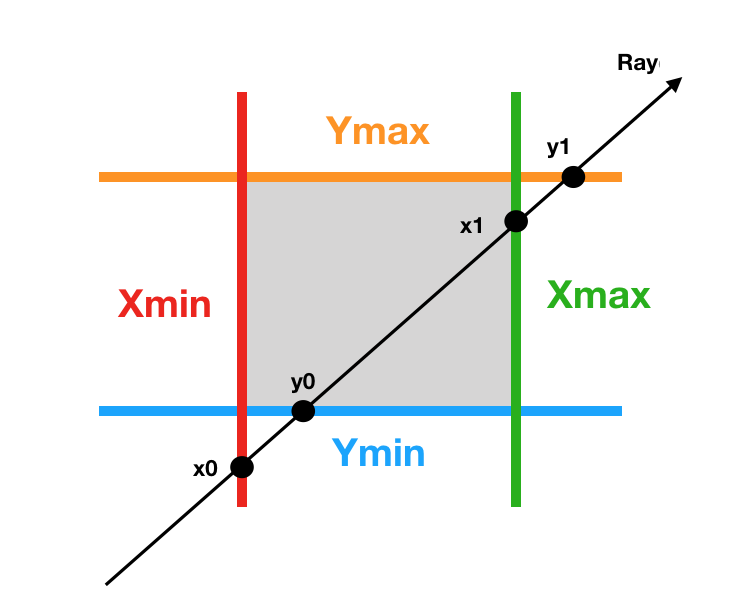
\includegraphics[width=\linewidth]{AABB}
%		\caption{Ray/box intersection in 2D}
%		\label{AABB}
%	\end{subfigure}
%	\qquad
%	\begin{subfigure}{0.4\textwidth}
%		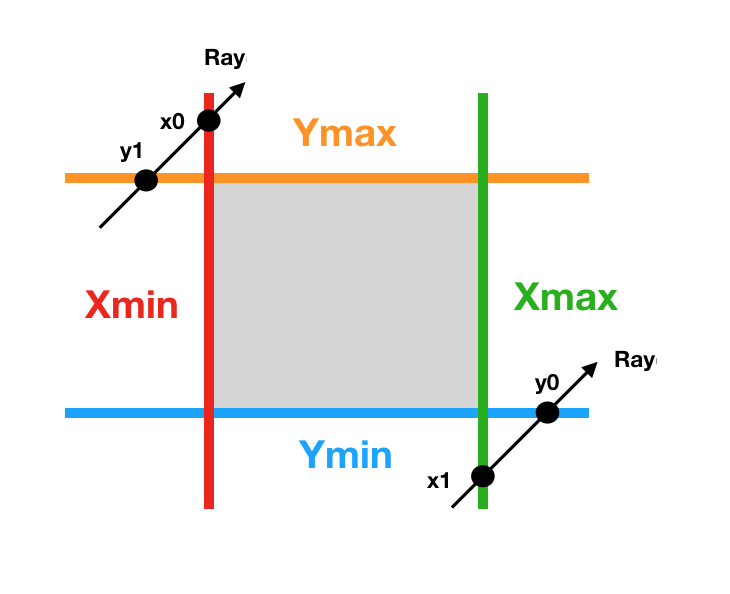
\includegraphics[width=\linewidth]{AABB2}
%		\caption{No intersection}
%		\label{AABB2}
%	\end{subfigure}
%	\caption{Illustrations of the ray/box intersection in 2D}
%\end{figure}
%%
%We understand from the figures \ref{AABB} and \ref{AABB2} that we will be able to determine if a ray intersects a box by comparing the coordinates of the points of intersection with the planes. Notably, if $x_0 > y_1$ or $y_0 > x_1$ the ray will not intersect the box (see fig. \ref{AABB2}). Otherwise, the same principle will apply on $z$. There will then be no intersection if $max(x_0 ; y_0) > z_1$ or $ z_0 > min(x_1 ; y_1)$. Note that if the ray is directed in the opposite direction, the $\alpha_0$ and $\alpha_1$ have to be inverted ($\alpha$ corresponding to the coordinates $x,y,z$).

We can can then measure the computation time of one iteration (i.e all rays are intersecting a triangle) by increasing the number of rays and the number of faces in the mesh. As we can see in the figure \ref{times} the complexity of the algorithm is almost linear by using the octree method. This allows to treat large meshes with millions of rays by maintaining a low computation time. In particular, we can see in the table \ref{tabComplexite} that for 250~000 rays and faces the computation time is divided by 1000 by using the octree. 

\begin{figure}[h]
\centering
	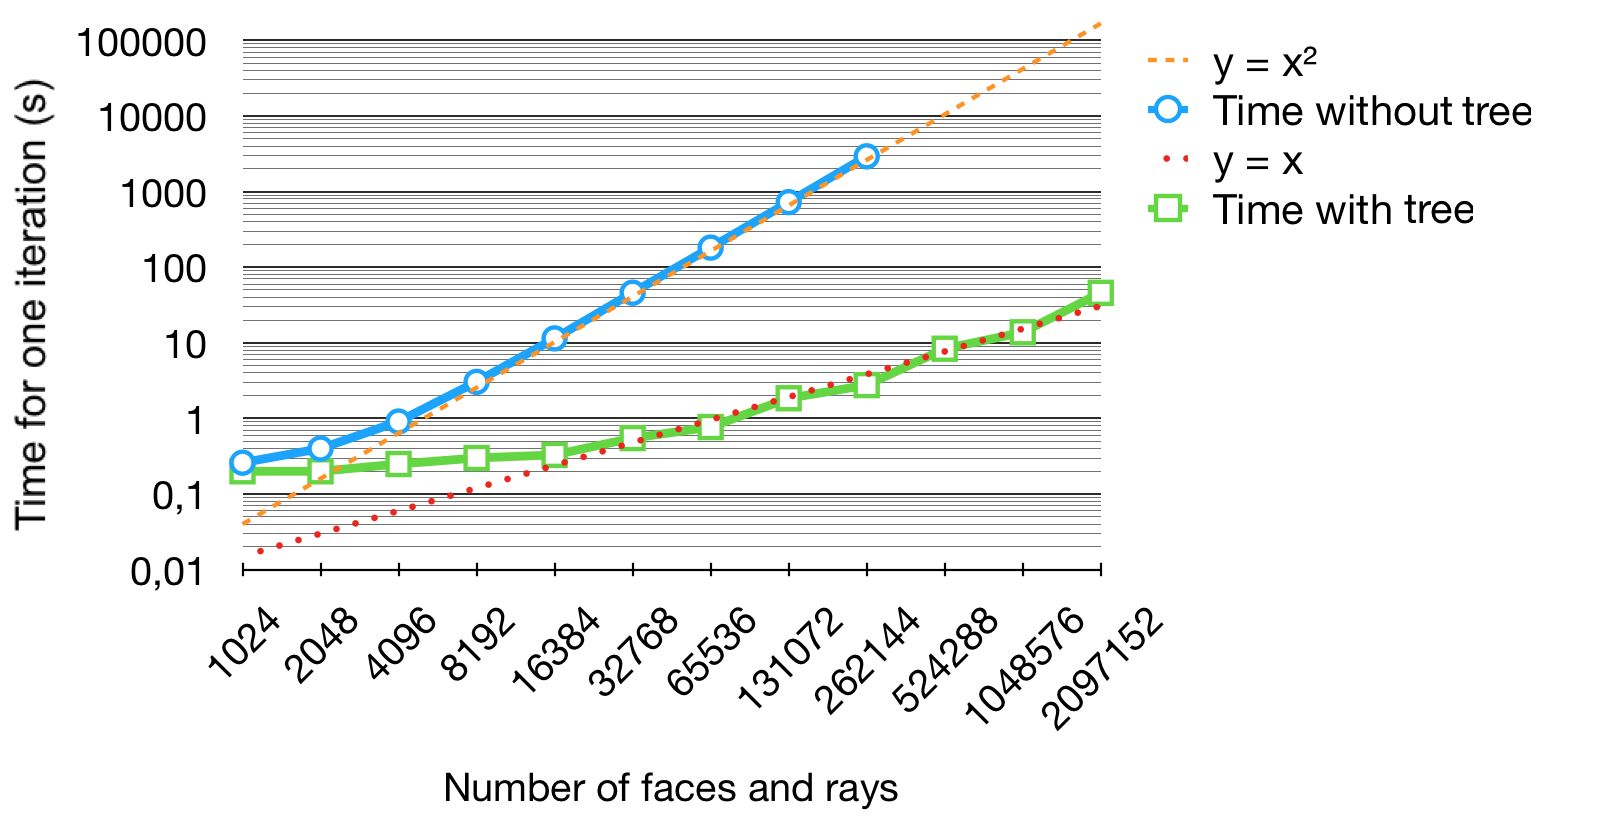
\includegraphics[width=0.8\linewidth]{times}
	\caption{Computation time for one iteration and $N = M$ (log scale)}
	\label{times}
\end{figure}
%
\begin{table}[h]
\centering
	\begin{tabular}{| c | c | c |}
		\hline
		Number of faces and rays & Time \textbf{without} Octree (s) & Time \textbf{with} Octree (s)\\
		  \hline
		  \hline
		   $2^{10}$ (=1~024) & 0,26 &	0,2 \\
		   \hline
		$2^{11}$ (=2~048)  & 0,4	& 0,2 \\
		   \hline
		$2^{12}$ (=4~096) & 0,91	& 0,25\\
		   \hline
		$2^{13}$ (=8~192) & 3,05 &	0,3\\
		   \hline
		$2^{14}$ (=16~384) & 11,44	&0,33\\
		   \hline
		$2^{15}$ (=32~768) & 46,02	&0,55 \\
		     \hline
		    $2^{16}$ (=65~536) & 181,61	& 0,77\\
		   \hline
		$2^{17}$ (=131~072) & 725,17	& 1,85\\
		\hline
		$2^{18}$ (=262~144) & 2927,9 & 2,76 \\
		\hline
		$2^{19}$ (=524~288) & X & 8,36 \\
		\hline
		$2^{20}$ (=1~048~576) & X & 13,78 \\
		\hline
		%$2^{21}$ (=2~097~152) & X & 45,83 \\
		%\hline
	 \end{tabular}
	\caption{Computation time for one iteration and $N = M$}
	\label{tabComplexite}
\end{table}


\newpage

\section{Validation}\label{sec5}

In order to validate our approach and our method we compare the experimental results with theoretical results. 

\subsection{Quadratic decrease}
First, to validate the quadratic decrease of the energy (see section \ref{sec2}) we observe the room impulse response of a cubic room whose all walls are 100\% absorbant except the walls on the x-axis (this may remind a Fabry-P\'erot interferometer). This particular room stands for a free space simulation where the distance between the source and the receiver is regularly increased. Furthermore, since the rays spread on the x-axis and -x-axis and return in phase, the number of rays received is twice the number of rays in free space.
%
\begin{figure}[h]
\centering
	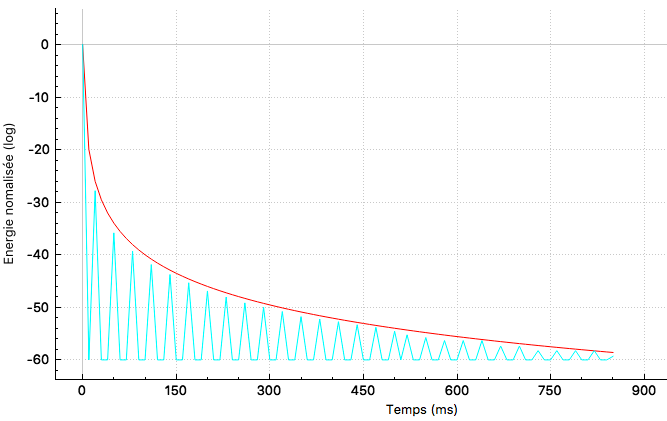
\includegraphics[width=0.6\linewidth]{test1}
	\caption{RIR in a Fabry-P\'erot-like configuration for 3 millions of rays (blue) sampled at 100Hz and $f(x)=\frac{2}{x^2}$ (red)}
	\label{test1}
\end{figure}
%
The room impulse response (see fig. \ref{test1}) follows the function $f(x)=\frac{2}{x^2}$ which is the expected behavior. In free space, the number of rays collected stands for the surfaces ratio and the quadratic decrease :
\begin{equation}
\frac{n}{N} = \frac{\int_s dS}{\int_{\sigma} dS} = \frac{\pi r^2}{4\pi d^2},
\end{equation}
with :
\begin{itemize}
\item$n$ : the number of rays collected,
\item$N$ : the total number of rays,
\item$s$ : the constant surface of the receiver (disk) collecting rays,
\item$\sigma$ : the emission sphere surface,
\item$r$ : the constant radius of the receiver,
\item$d$ : the emission sphere radius (i.e the distance between the source and the receiver).
\end{itemize}

\subsection {Energy conservation}
The second test allows to simulate the conservation of the energy. We use a 100\% reflecting sphere (2m radius) pretty well refined (300~000 faces) and position the source and the receiver in the center. At each iteration all the rays refocus in the center of the sphere and then are captured by the receiver.
\begin{figure}[h]
\centering
	\begin{subfigure}{0.45\textwidth}
		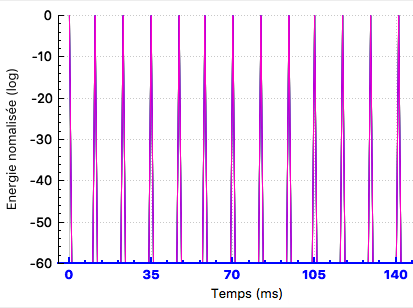
\includegraphics[width=\linewidth]{test2RIR}
		\caption{RIR for a 100\% reflecting sphere - 12 iterations}
		\label{test2RIR}
	\end{subfigure}
	\quad
	\begin{subfigure}{0.38\textwidth}
		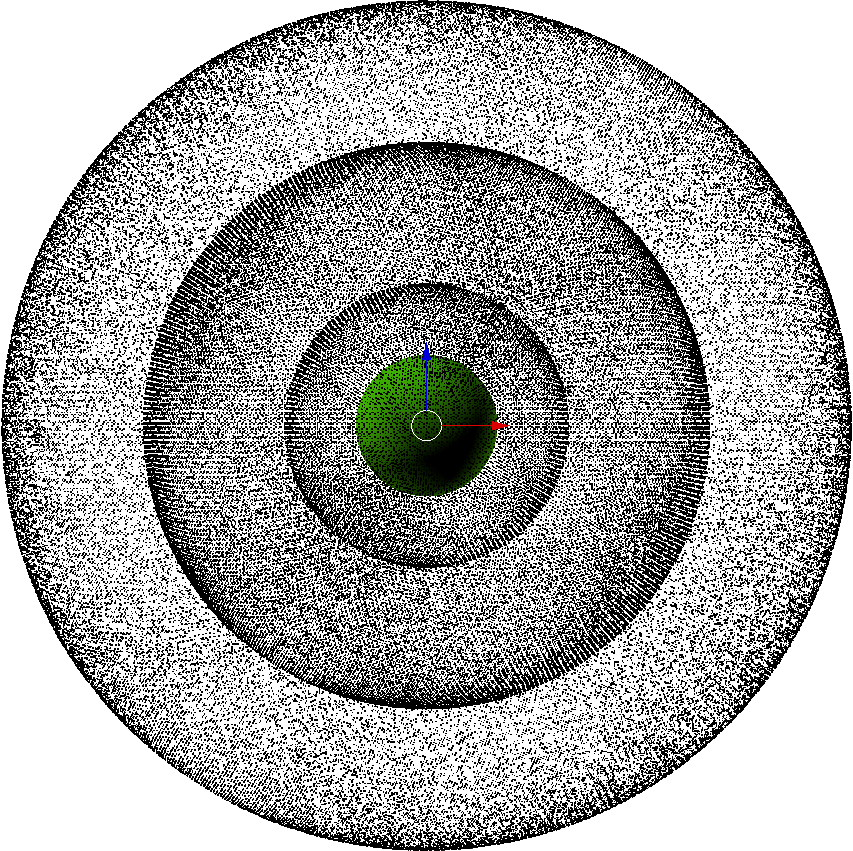
\includegraphics[width=\linewidth]{test2SI}
		\caption{Position of the images-sources - 4 iterations}
		\label{test2SI}
	\end{subfigure}
	\caption{100\% reflecting sphere}
\end{figure}
%
We observe the expected result as the room impulse response is a Dirac comb (see fig. \ref{test2RIR}) and the image-sources are positioned on spheres whose radius doubles at each iteration (see fig. \ref{test2SI}).
%
\begin{figure}[h]
\centering
	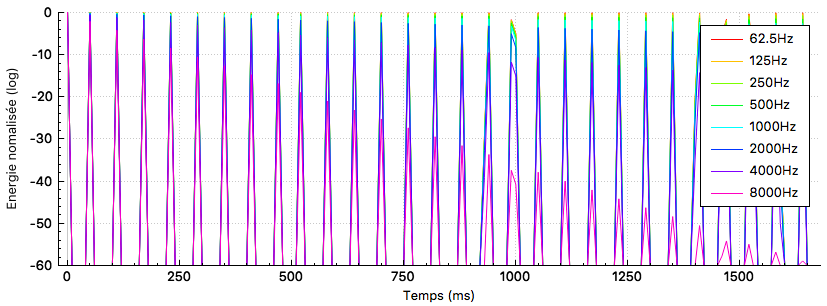
\includegraphics[width=0.6\linewidth]{test2absair}
	\caption{RIR for a 100\% reflecting sphere with air absorption - 30 iterations}
	\label{test2absair}
\end{figure}
%
By adding the air absorption (see fig. \ref{test2absair}) we can observe that the highest frequencies decrease faster than the lowest which reflect the nature behavior.

\subsection{Shoe box case}
To finalize the validation algorithm we compare the results of a shoe box type room with an analytic computation. The image-sources can be positioned in space with the following formula \cite{mcgovern} :
\begin{align}
P_{is} = i \times D + P_s \times (-1)^i,
\end{align}
with : 
\begin{itemize}
\item$i \in (-n, n)$ and $n \in \mathbb{N}$,
\item$P_{is}$ : the image-source position coordinate on X, Y or Z,
\item$P_s$ : the source position coordinate on X, Y or Z,
\item$D$ : the room dimension on X, Y or Z.
\end{itemize}
The energy of each image-source is $\frac{1}{d^2}$ where $d$ is the distance between the image-source avec the receiver. If we compare the position of these theoretical image-sources with the image-sources obtained with the algorithm, we get the exact same result to the float precision ($10^{-6}m$). Concerning the energy, we compare two kind of errors : the relative error such as :
\begin{align}
\epsilon_{rel} = \frac{|E_{exp}-E_{theo}|}{E_{theo}},
\end{align}
and the infinity norm error which express the fact that the further away the image-source is from the receiver, the less important the error will be for the final result.
\begin{align}
\epsilon_{\infty} = \frac{|E_{exp}-E_{theo}|}{\max(E_{theo})}.
\end{align}
We can also add some absorption coefficient on the walls and take into account the air absorption. We can see in the figure \ref{test3_8} that the relative error of the energy image-source per image-source remains always below 5\%. In the same way we see in the figure \ref{test3_9} that the infinity norm error is below $0,3\%$ for all frequencies.

\begin{figure}[h]
\centering
	\begin{subfigure}{0.49\textwidth}
		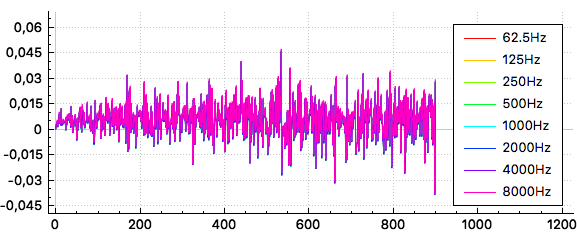
\includegraphics[width=\linewidth]{test3_8}
		\caption{Relative error}
		\label{test3_8}
	\end{subfigure}
	\begin{subfigure}{0.49\textwidth}
		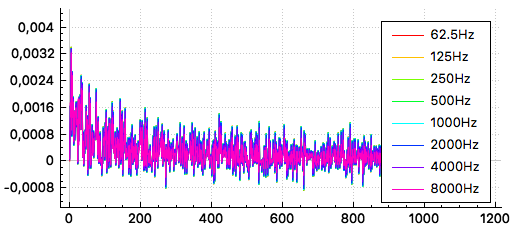
\includegraphics[width=\linewidth]{test3_9}
		\caption{Infinity norm error}
		\label{test3_9}
	\end{subfigure}
	\caption{Error for each image-sources with walls and air absorption - 1~000~000 rays}
\end{figure}


\newpage

\section{Developed softwares }\label{sec6}

The room acoustic tool is available in two forms. 

\subsection{Matlab library}
First a Matlab library \cite{gypsilab} ... \\

\subsection{Blender add-on}
In a second hand the tool is also available as a Blender add-on. The user can work on the CAD software to model the room under test, positioning the sources and the receiver and assign materials to the walls. By clicking on the "Run" button, the mesh is exported, the materials are linked to eight absorption coefficients (extracted from a data base) and the acoustic calculation tool is launched. This is an executable C++ complied software which treats information form Blender and generates the room impulse response. The communication between the CAD and the executable is done thanks to an .obj file, so using Blender is not necessary. Different options allow to analyse the results by reimporting rays or image-sources on the CAD software. It is also possible to listen an audio file convolved to the RIR to listen the reverberate sound.


%\begin{figure}
%	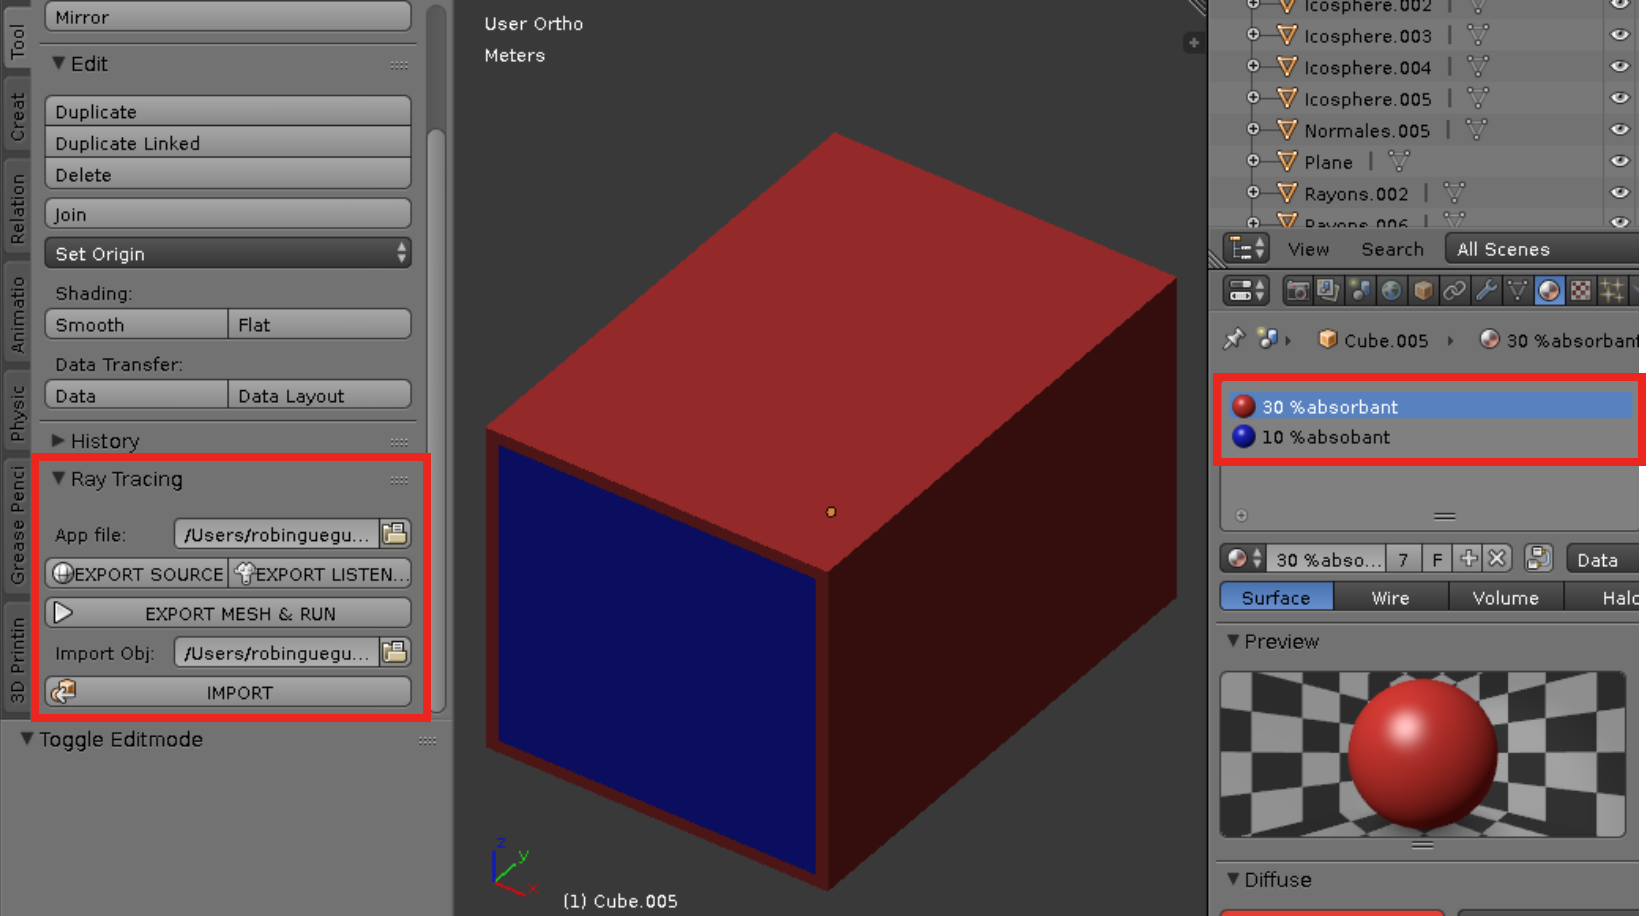
\includegraphics[width=\linewidth]{add-on}
%	\caption{Add-on Blender}
%\end{figure}

\begin{figure}[h]
\centering
	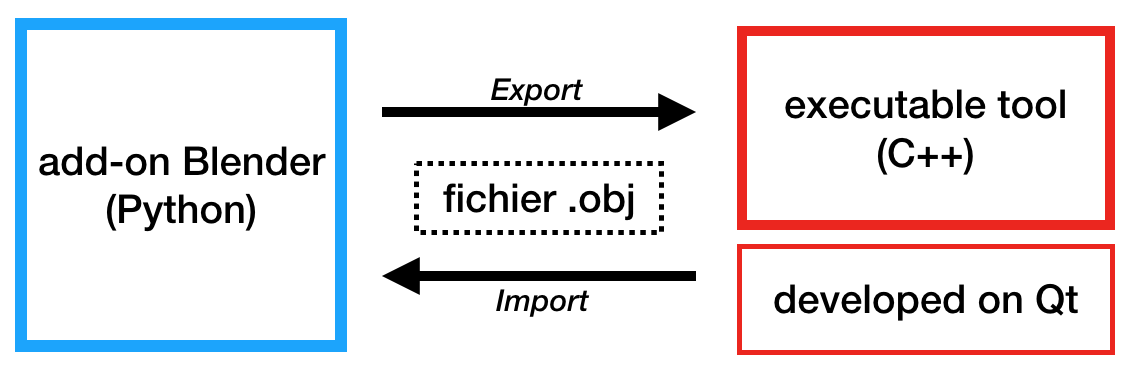
\includegraphics[width=0.5\linewidth]{software}
	\caption{Software architecture}
\end{figure}

\begin{figure}[h]
\centering
	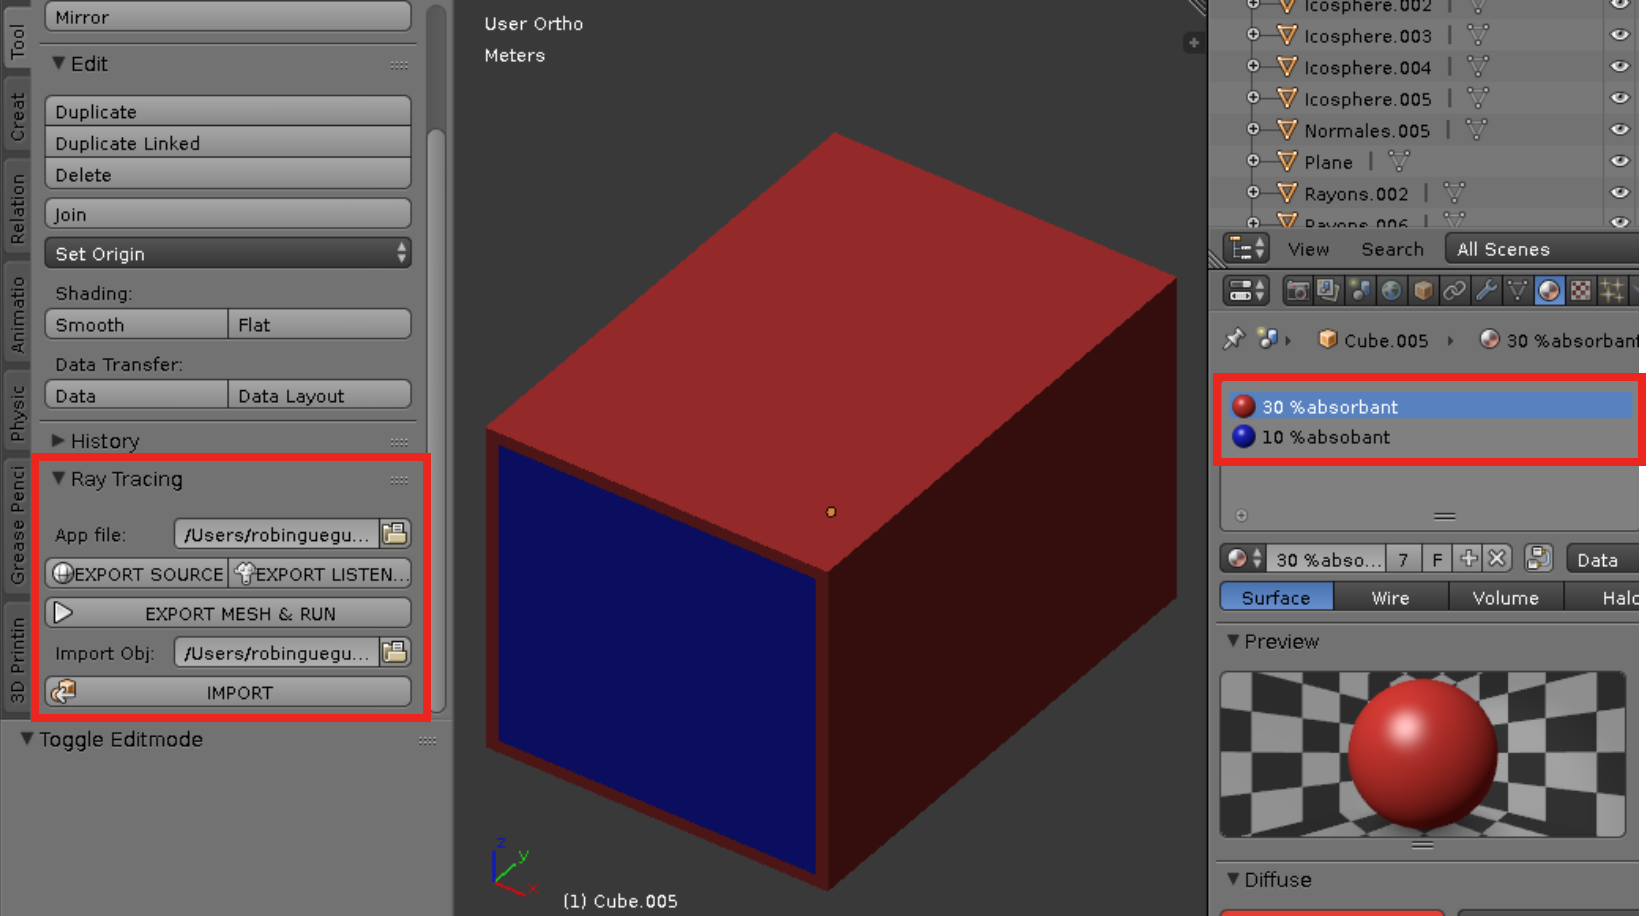
\includegraphics[width=0.8\linewidth]{add-on}
	\caption{Add-on Blender for exporting/importing meshes and running computation tool}
	\label{add-on}
\end{figure}


\section{Application to the antic theatre of Orange}\label{sec7}

\begin{figure}[h]
\centering
	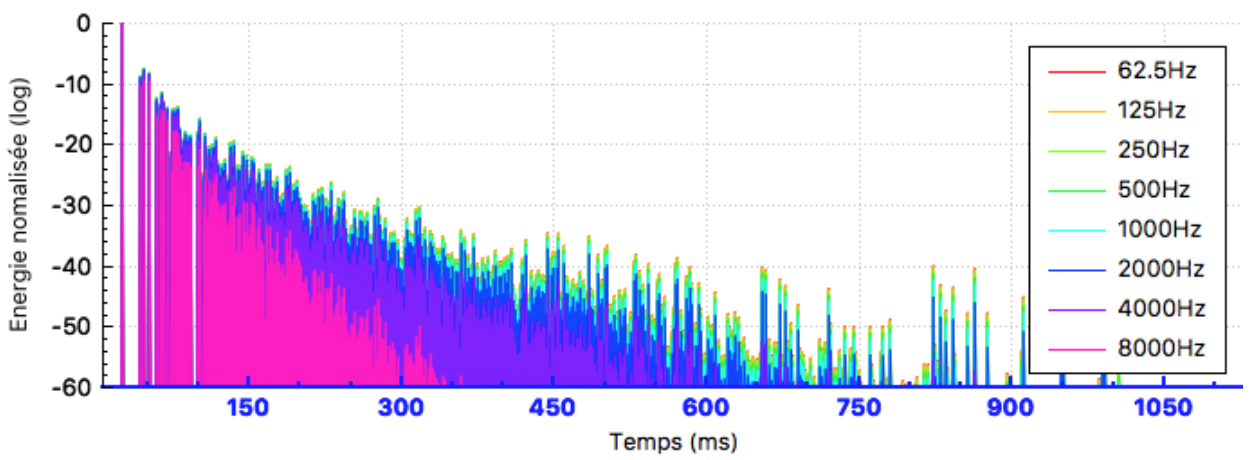
\includegraphics[width=0.7\linewidth]{rir}
	\caption{Room impulse response of the antic theater of Orange}
	\label{rir}
\end{figure}

The acoustic simulation can be done on the ancient theater of Orange. Because it is an open room the software automatically add a 100\% absorbant box around the building to be sure to always count all rays. We can then calculate the image-sources and the RIR for different configurations of the theatre or different materials. Indeed, archeologists want to explore some architecture hypothesis from missing part of the theatre. An acoustical analysis can allow to understand some behaviors like : the influence of the position of the spectators in the bleachers, the shape of the roof, the materials of the \textit{orchestra}, etc. With a 600~000 faces theatre (i.e including decoration elements of the stage wall), the RIR at $RT_{60}$ is generated in 20 minutes for one million rays (see fig. \ref{rir}). Each iteration is done in 25s so it really depends on the materials chosen. We can note that the more details of the mesh are refined the more we can simulate diffraction effect. Indeed, in high frequency, small detail elements will be able to reflect the rays in different directions which can resemble diffraction effects. In the theater it will be really interesting to study where the reflection come from. Thus, we project the image-sources on the wall of the theater to understand what wall is the main contributor to the energy received (see fig. \ref{theatre}).

\begin{figure}[h]
\centering
	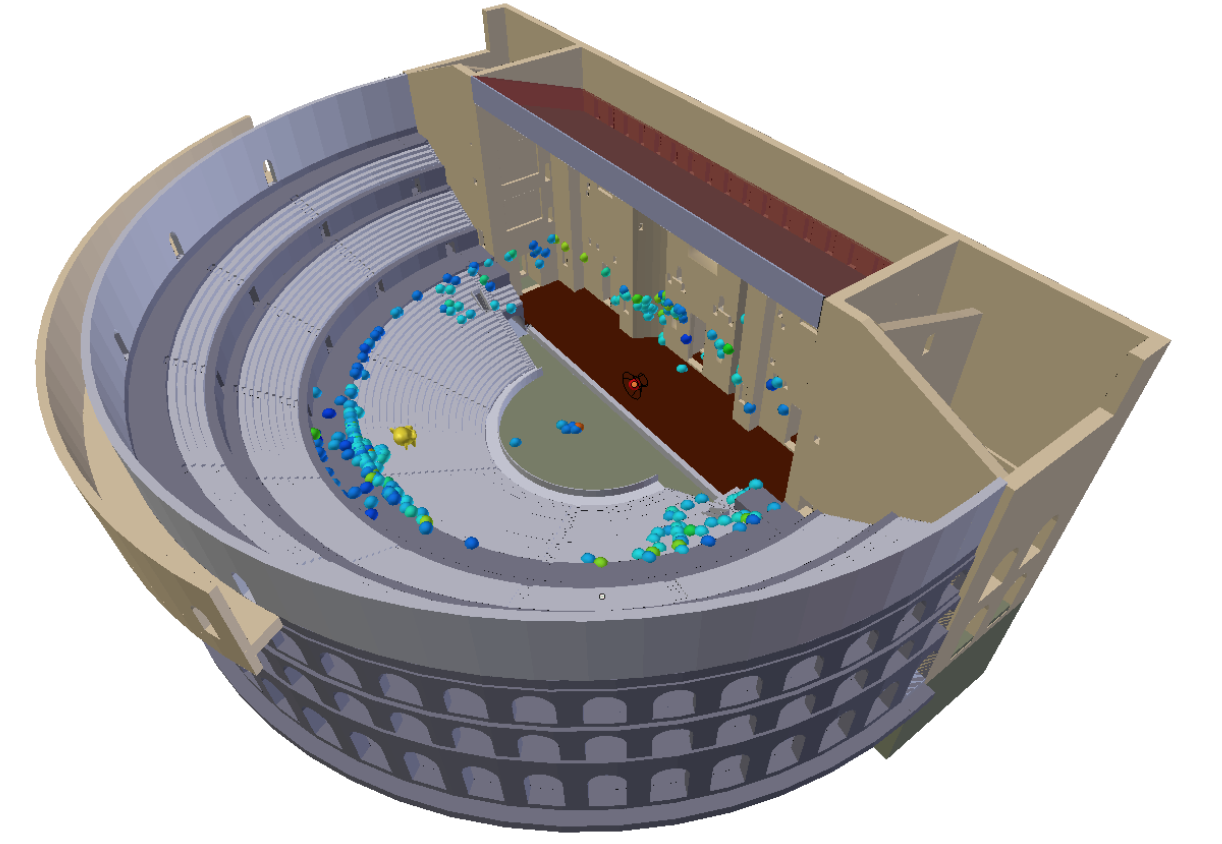
\includegraphics[width=0.7\linewidth]{theatre}
	\caption{Images-sources projected on the theatre of Orange}
	\label{theatre}
\end{figure}


\section{Conclusions}

We presented the problems raised by an acoustic study of an ancient monument. The complex geometry of this type of building and their colossal size requires the use of approximate calculation methods. Thus, by simulating the reflections and absorptions of the walls, it is possible to study the reverberation of a room. Despite the inevitable approximations of the model, we have proved that the laws of physics are respected. A fast algorithm has been implemented to allow users to easily and quickly test their architectural assumptions. Thus, the calculation time becomes linear to the product number of mesh elements/number of rays. The algorithm developed allows the study of the temporal graph of reverberation of the building as well as the position in space of the various sound reflections. Furthermore, a sound signal could be heard in three dimensions thanks to binaural filters and steering control can be done with "Head Tracker" mounted on a headset.

However, there are many opportunities for improvement that remain under consideration for this type of software tool. First, in a context where virtual reality is becoming more and more important in today's applications, we could consider moving the listener in real time and thus, allow a complete virtual tour of the building. Secondly, from the point of view of the analysis results, there are many possible improvements at the graphic level. That raises some questions. How to view acoustic calculation results? What information is essential for an archaeologist wishing to study the acoustics of a monument? Similarly, is it essential to add diffraction effects to the model? If so, what is the best method? Could certain acoustic behaviours be treated locally and then inserted into the model by ray tracing? Finally, it would also be interesting to use sources whose directivity is not uniform. This would be more representative of the real cases, and in particular, of the use made in Orange at the theatre origin. The sounds were then emitted by musical instruments or by the human voice possibly amplified by a mask.



\section*{Acknowledgments}
The authors would particularly like to thank Fran\c{c}ois Alouges, Titien Bartet, Pascal Frey and Emmanuelle Rosso for all the help they each provided at the different stages of this project. Thanks also to Jean-Dominique Polack for his wise advice on architectural acoustics.

%\subsection*{Author contributions}
 

%\subsection*{Financial disclosure}


%\subsection*{Conflict of interest}



%\section*{Supporting information}

%The following supporting information is available as part of the online article:
%
%\noindent
%\textbf{Figure S1.}
%{500{\uns}hPa geopotential anomalies for GC2C calculated against the ERA Interim reanalysis. The period is 1989--2008.}
%
%\noindent
%\textbf{Figure S2.}
%{The SST anomalies for GC2C calculated against the observations (OIsst).}


%\section{Glossary\label{app1}}

%\printglossaries


	

	
		
%Use \verb+\begin{verbatim}...\end{verbatim}+ for program codes without math. Use \verb+\begin{alltt}...\end{alltt}+ for program codes with math. Based on the text provided inside the optional argument of \verb+\begin{code}[Psecode|Listing|Box|Code|+\hfill\break \verb+Specification|Procedure|Sourcecode|Program]...+ \verb+\end{code}+ tag corresponding boxed like floats are generated. Also note that \verb+\begin{code}[Code|Listing]...+ \verb+\end{code}+ tag with either Code or Listing text as optional argument text are set with computer modern typewriter font.  All other code environments are set with normal text font. Refer below example:
%
%\begin{lstlisting}[caption={Descriptive Caption Text},label=DescriptiveLabel]
%for i:=maxint to 0 do
%begin
%{ do nothing }
%end;
%Write('Case insensitive ');
%WritE('Pascal keywords.');
%\end{lstlisting}
%
%
%
%\subsection{Subsection title of first appendix\label{app1.1a}}
%
%\noindent\textbf{Unnumbered figure}
%
%
%\begin{center}
%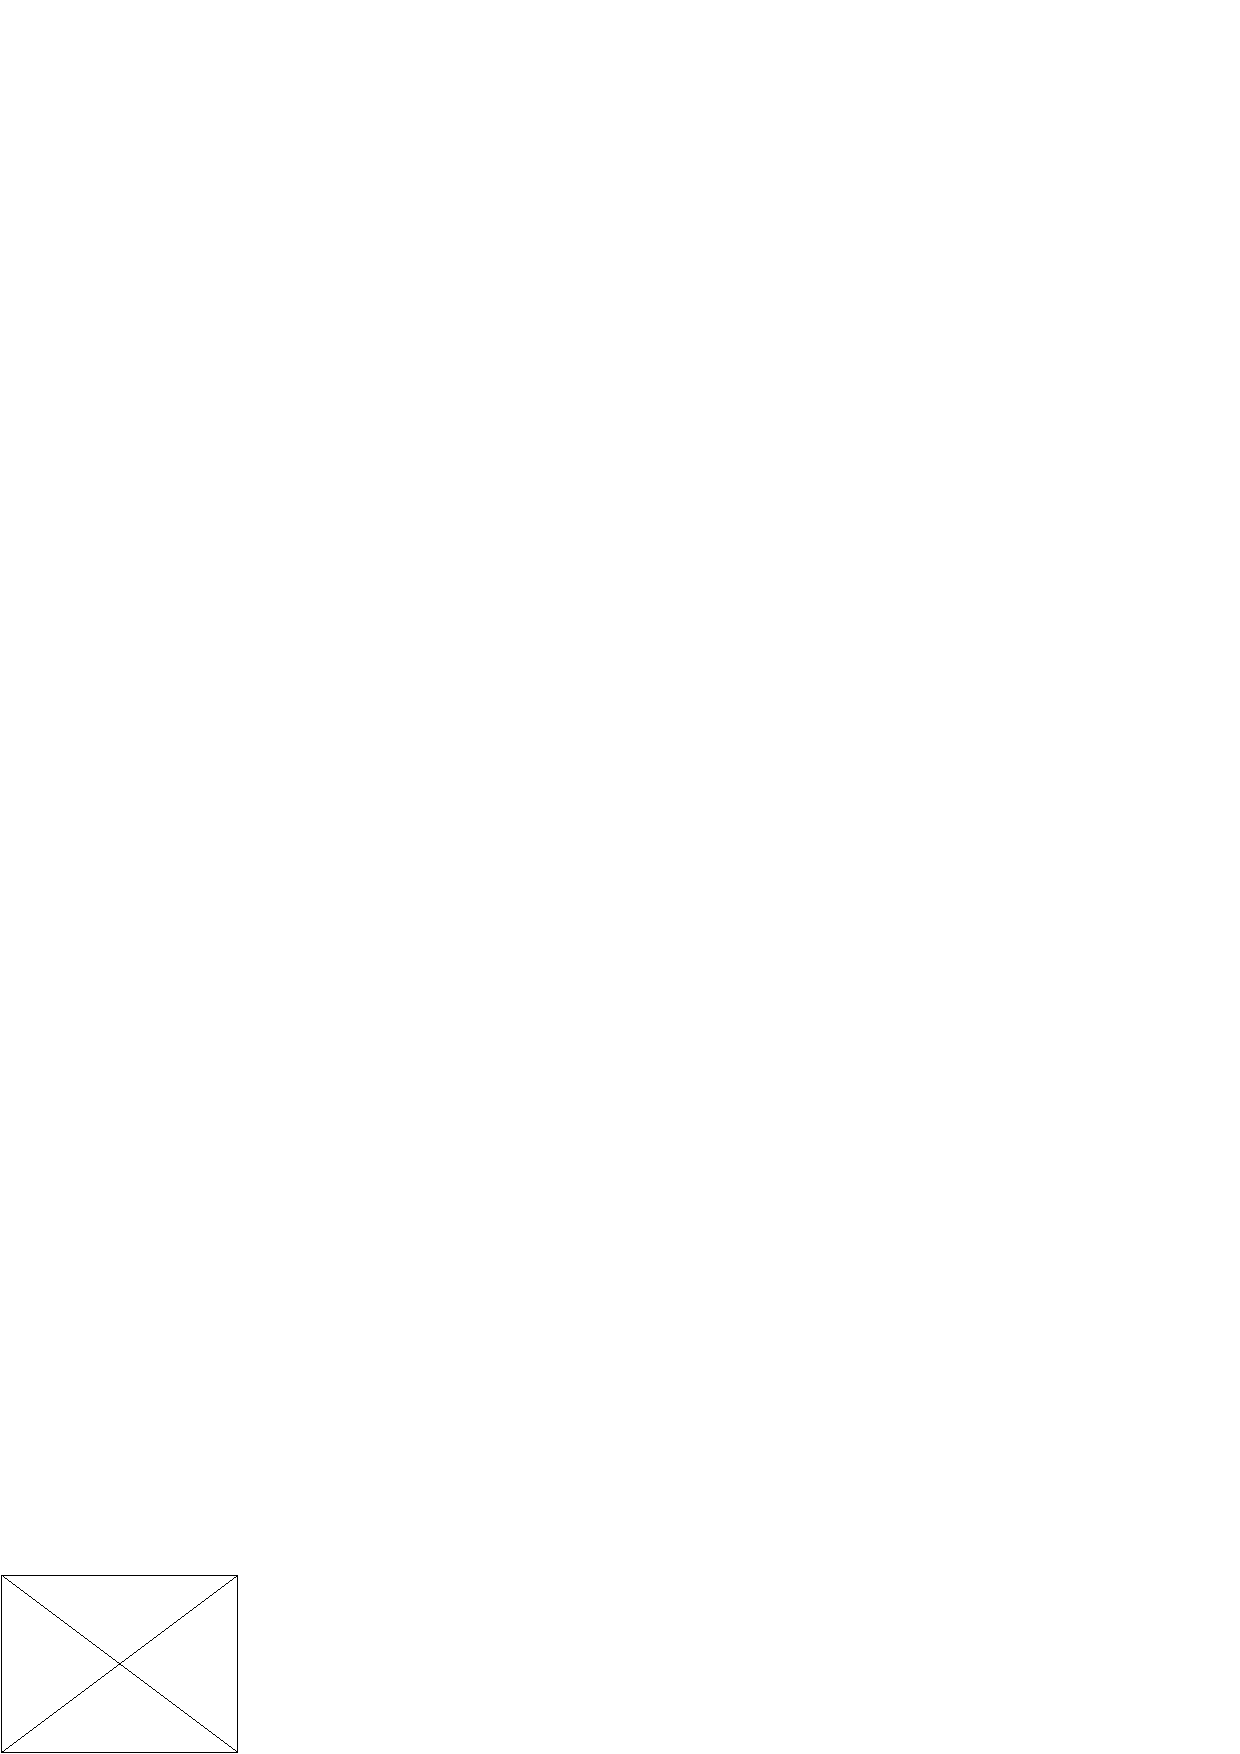
\includegraphics[width=7pc,height=8pc,draft]{empty}
%\end{center}
%
%
%%== Figure 4 ==
%%% Example for figure inside appendix
%\begin{figure}[t]
%\centerline{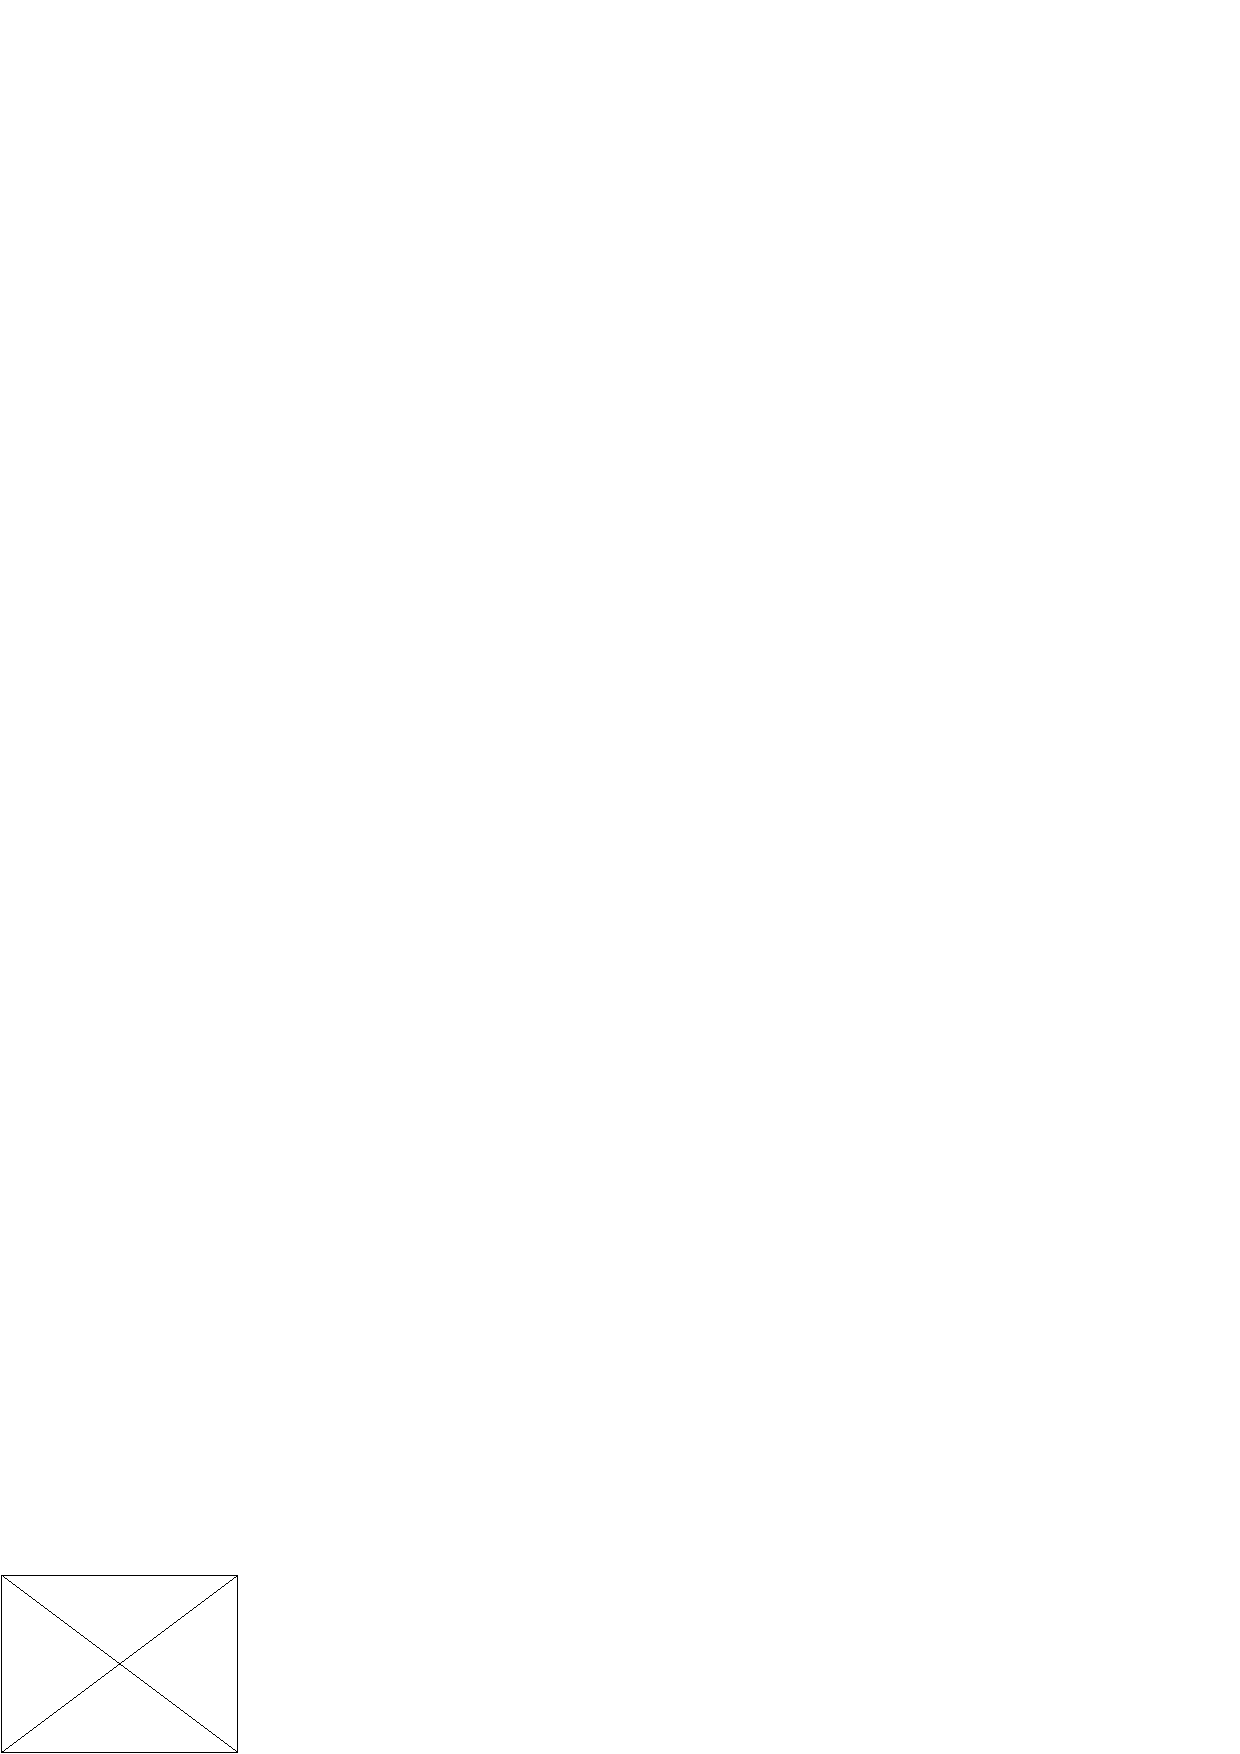
\includegraphics[height=10pc,width=78mm,draft]{empty}}
%\caption{This is an example for appendix figure.\label{fig5}}
%\end{figure}


%\nocite{*}% Show all bib entries - both cited and uncited; comment this line to view only cited bib entries;
\bibliography{Biblio}%

\clearpage

%\section*{Author Biography}

%\begin{biography}{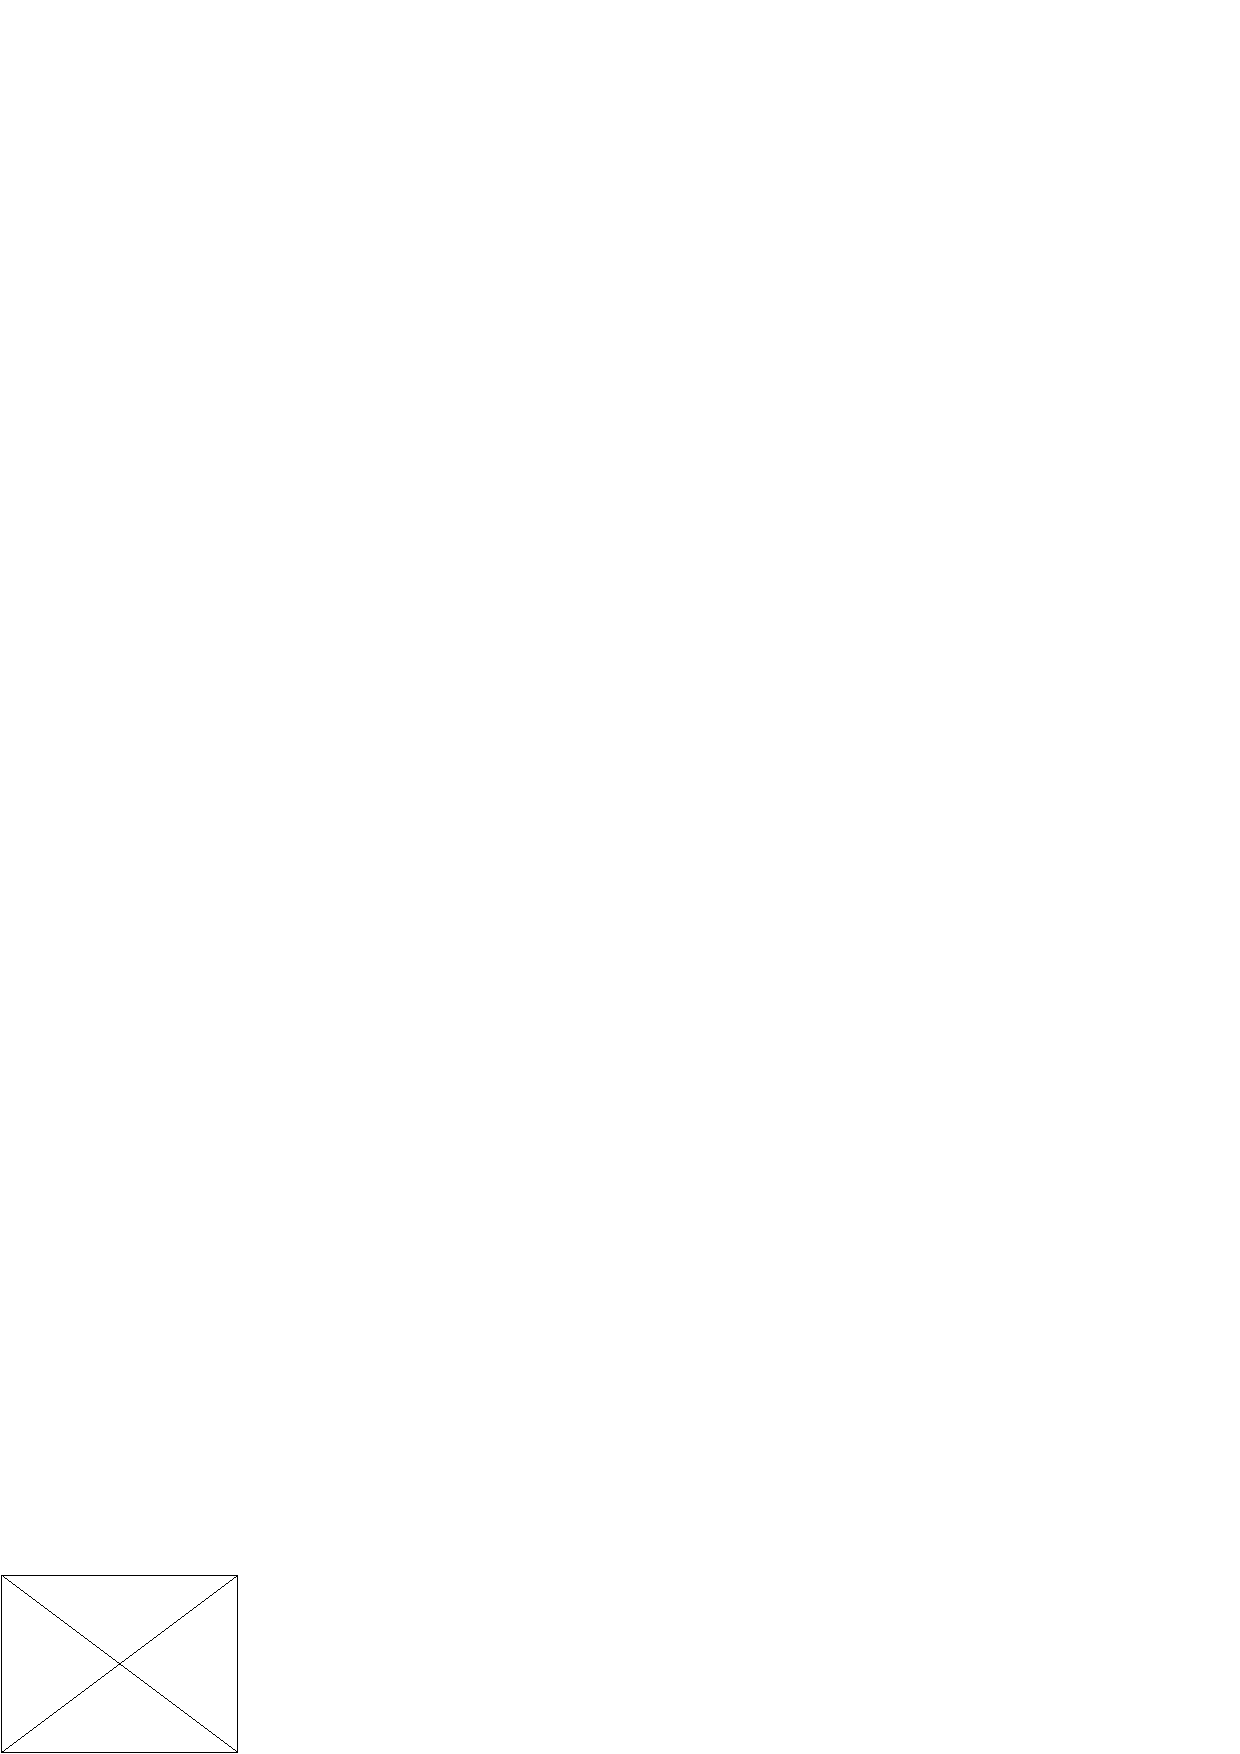
\includegraphics[width=66pt,height=86pt,draft]{empty}}{\textbf{Author Name.} This is sample author biography text this is sample author biography text this is sample author biography text this is sample author biography text this is sample author biography text this is sample author biography text this is sample author biography text this is sample author biography text this is sample author biography text this is sample author biography text this is sample author biography text this is sample author biography text this is sample author biography text this is sample author biography text this is sample author biography text this is sample author biography text this is sample author biography text this is sample author biography text this is sample author biography text this is sample author biography text this is sample author biography text.}
%\end{biography}

\end{document}
